% Wczytanie szablonu
\documentclass[nostrict]{Szablon}

% Definicja dokumentu
\usepackage[unicode=true]{hyperref}
\usepackage{listings}
\usepackage{array}
\usepackage{courier}
\newcommand\PDFtitle{Tytuł pracy}
\newcommand\PDFauthors{Imie Nazwisko}
\hypersetup{
  pdftitle={\PDFtitle},
  pdfauthor={\PDFauthors},
}

\addbibresource{bib.bib}

% Zmiana czcionki dla symulacji maszynopisu (verbatim)
\makeatletter
\renewcommand{\verbatim@font}{\ttfamily\small}
\makeatother

\usepackage{xcolor}
\usepackage{pdfpages}

%New colors defined below
\definecolor{codegreen}{rgb}{0,0.6,0}
\definecolor{codegray}{rgb}{0.5,0.5,0.5}
\definecolor{codepurple}{rgb}{0.58,0,0.82}
\definecolor{backcolour}{rgb}{0.95,0.95,0.92}
\newcommand{\magenta}[1]{\textcolor{magenta}{#1}}
%Code listing style named "mystyle"
\lstdefinestyle{mystyle}{
  backgroundcolor=\color{backcolour}, commentstyle=\color{codegreen},
  keywordstyle=\color{magenta},
  numberstyle=\tiny\color{codegray},
  stringstyle=\color{codepurple},
  basicstyle=\ttfamily\footnotesize,
  breakatwhitespace=false,         
  breaklines=true,                 
  captionpos=b,                    
  keepspaces=true,                 
  numbers=left,                    
  numbersep=5pt,                  
  showspaces=false,                
  showstringspaces=false,
  showtabs=false,                  
  tabsize=2
}

%"mystyle" code listing set
\lstset{style=mystyle}
% Część właściwa pracy
\begin{document}
\frontmatter
%\includepdf[pages=-,fitpaper]{}    % Title page, add pdf filename in brackets
\chapter*{Streszczenie}
\addcontentsline{toc}{chapter}{Streszczenie}
Tematem pracy inżynierskiej jest realizacja gry z gatunku strategii czasu rzeczywistego osadzonej w realiach historycznych
wybranej epoki. Niniejsza praca zawiera opis przykładowych rozwiązań zastosowanych w niektórych grach dostępnych na rynku
oraz projekt i implementację wytwarzanego programu. Praca skupia się na przedstawieniu zaimplementowanych mechanik oraz
sposobie oddania realiów, w których osadzona jest fabuła opracowanej gry.

Do przygotowania prototypu gry wykorzystano silnik Unity oraz udostępniane przez niego narzędzia. Za ich pomocą
przygotowano podstawowe mechanizmy, typowe dla gier strategii czasu rzeczywistego oraz przykładowe zadania tworzące
fabułę gry. Utworzony prototyp pozwala na dalsze rozwijanie świata gry poprzez dodawanie nowych zadań oraz elementów
rozgrywki. Zagadnienia implementacyjne zostały opisane w rozdziale Implementacja, a efekt finalny w Przebiegu rozgrywki.

Podstawowym celem projektu jest przygotowanie gry, która w jak najdokładniejszy sposób oddawałaby realia wybranej epoki.
Zdecydowaliśmy się na osadzenie fabuły we wczesnym średniowieczu. Główną inspiracją stali się Celtowie, którzy w
tamtych czasach zamieszkiwali tereny współczesnej Irlandii. W ramach projekty przede wszystkim skupiono się na
opracowaniu sposobu nawigacji w grze oraz zachowania przeciwników, stosujących broń oraz słownictwo charakterystyczne
dla realiów historycznych. W rozdziale Projekt została przedstawiona wizja autorów na poszczególne elementy gry.

W celu przygotowania się do projektu i implementacji gry, przeprowadzono przegląd wybranych mechanik w grach dostępnych
na rynku. Niniejsza praca zawiera opis ich działania na podstawie przykładów z istniejących gier oraz sposobu, w jaki
wpływają na ich rozgrywkę. Przedstawione rozwiązania stanowią inspirację dla wytwarzanej gry.

Praca została przygotowana przez trzech współautorów. Bartosz Strzelecki był odpowiedzialny za rozdziały ref{ss:rts}, ...
Jest również współatorem punktów ref{ss:comp} oraz ... Bogna Lew odpowiadała za rozdziały ref{ss:rpg}, ref{s:budowanie},
ref{s:walka}, ... oraz współtworzyła ref{ss:comp}, {chap:introduction}, ... Zofia Sosińska była odpowiedzialna za
pracę nad rozdziałami ref{ss:tbs}. Współtworzyła również rozdział {chap:introduction}.

\chapter*{Abstract}
\addcontentsline{toc}{chapter}{Abstract}  
The topic of the enginnering thesis is a prototype of real-time strategy game set in historical reality of selected era.
This work contains a description of sample solutions used in selected games available on the market
and the design and a overview of the implementation of the produced program. The work focuses on the presentation 
of the implemented mechanics as well as
the way of rendering the realities in which the plot of the developed game is set.

The Unity engine and the tools it provides were used to prepare a prototype of the game.
Employing these tools, basic mechanics typical of real-time strategy games, were prepared,
as well as sample tasks forming the games's plot. The devised prototype allows for 
further development of the game environment by adding new activities and gameplay elements.
The implementation matters are described in the Implementation chapter, and the results in the Gameplay Course.

The fundamental goal of the project is to develop a game that would reflect the reality of the selected era as accurately as possible.
The main inspiration came from the Celts, who at that time inhabited the territory of modern day Ireland. 
The project primarily focused on
developing the means of navigation in the game and the behavior of opponents, using weaponry and vocabulary characteristic to the
historical realities. The Project chapter presents the authors' vision for the various elements of the game.

In preparation for the design and implementation of the game, a review of selected mechanics in games available
on the market were conducted. This paper describes how they work using examples from existing games and how
they affect their gameplay. The solutions presented provide inspiration for the developed game.

\chapter*{Spis treści}
\addcontentsline{toc}{chapter}{Spis treści}

\tableofcontents

\mainmatter
\chapter*{Wykaz ważniejszych oznaczeń i skrótów}
\addcontentsline{toc}{chapter}{Wykaz ważniejszych oznaczeń i skrótów}
\begin{description}[style=multiline,leftmargin=3cm]
\item[RTS] Gra strategii czasu rzeczywistego (ang. \textit{real-time strategy}). Jest to gatunek gier, w którym gracz nie jest
ograniczany przez turowość i kolejność ruchów. Wymusza szybsze podejmowanie decyzji, a ich skutki są natychmiastowe.
\item[cRPG] Kompyterowa gra fabularna (ang. \textit{computer role-playing game}). Gatunek gier, w którym gracz wciela
się w postać lub drużynę, przemieszczając się w świecie stworzonym przez autorów gry.
\item[TBS] Strategiczna gra turowa (ang. \textit{turn-based strategy}). Jest to podgatunek gier strategicznych, w którym
gracze wykonują swoje akcje w turach.
\item[AAA (Triple-A)] Termin stosowany w przemyśle gier komputerowych. Służy do określenia wysokobudżetowych gier, od
których oczekuje się wysokiej jakości.
\item[Wielkie odkrycia geograficzne] Termin odnoszący się do odkryć geograficznych, które miały miejsce na przełomie XV
i XVI wieku.
\item[AI] Sztuczna inteligencja (ang. \textit{artificial intelligence}) jest wykorzystywana do imitowania inteligentnego
zachowania postaci niezależnych.
\item[NPC] Termin określa postacie niezależne (ang. \textit{non-playable character}), czyli postacie, które nie są kontrolowane bezpośrednio
przez gracza.
\item[Input Manager] Komponent silnika Unity, który umożliwia definiowanie wirtualnych osi oraz przypisywanie do nich
odpowiednich klawiszy. Poprzez odczyt wartości zwracanej przez oś możliwe jest wyznaczenie odpowiedniej akcji.
\item[UI] Interfejs użytkownika (ang. \textit{user interface}), czyli oprogramowanie umożliwiające użytkownikowi
interakcję z systemem.
\end{description}

\chapter{Wstęp i cel pracy}\label{chap:introduction}


\chapter{Przegląd strategii czasu rzeczywistego}

“Starożytni świat widzieli inaczej, mniej płasko”\cite{gbobrektvgry}. Dobrze obrazującym ówczesne postrzeganie przestrzeni przykładem jest mapa Imperium Rzymskiego,
pokazana na \ref{fig:mapaIR}. Czytanie jej dosłownie mija się z celem. Nie są na niej zachowane ani proporcje, ani strony świata. Mimo tego, że
basen Morza Śródziemnego został ówcześnie dosyć dokładnie oddany, “nie wydaje się, aby Rzymianom współczesna kartograficzna wierność była potrzebna”\cite{gbobrektvgry}.
“Dowódcy opierali się na swojej wiedzy, wiedzy wynajętych przewodników oraz informacjach zwiadowców i tubylców”\cite{gbobrektvgry}.
\begin{figure}[htbp]
    \centering
    \includegraphics[width=0.5\textwidth]{images/mapaIR.png}
    \caption{Mapa basenu Morza Śródziemnego z czasów Imperium Rzymskiego}\label{fig:mapaIR}
\end{figure}

Na odbiór gry wpływają zawarte w niej mechaniki. Twórcy bardzo częstostosują w nich uproszczenia, co ma na celu
ułatwienie graczowi wykonywanie zadań. Ma to jednak ogromny wpływ na zachowanie realizmu w grach, zwłaszcza tych opartych
na wydarzeniach historycznych oraz prawdziwym świecie. 

W niniejszym rozdziale zostały przedstawione wybrane mechaniki wykorzystywane w grach typu RTS. Omówione zostało ich
działanie na podstawie przykładów z wybranych gier. Celem tego jest obrazowe zaprezentowanie ich integralności
w grach oraz wpływu na rozgrywkę.

\section{Przegląd wybranych gatunków gier komputerowych}
W niniejszym podrozdziale zostały przedstawione wybrane gatunki gier komputerowych, które są najistotniejsze z punktu widzenia
projektu. Przede wszystkim zostały opisane gry typu strategii czasu rzeczywistego oraz strategiczne gry turowe TBS (ang.
\textit{turn-based strategy}. Ma to na celu zaprezentowanie podstawowych różnic pomiędzy tymi gatunkami.

"Gatunek określa graczowi, w jakiego typu grę będzie grał i jest bardzo przydatnym sposobem klasyfikacji gier"\cite{practical_game_design}.
Podział gier na gatunki pozwala na określenie podstawowych cech gry i daje ogólne pojęcie o jej charakterze. "Dlatego w
grach gatunek niesie więcej informacji niż temat i sceneria"\cite{practical_game_design}. Z tego powodu aby zrozumieć cel projektu ważne jest zauważenie podobieństw i różnic pomiędzy kluczowymi dla niego gatunkami.

\subsection{Specyfika gier RTS (Bartosz Strzelecki)}\label{ss:rts}

Strategie czasu rzeczywistego RTS (ang. \textit{real-time strategy}) odróżnia się od innych gatunków występowaniem zarówno strategicznych, jak i taktycznych
elementów rozgrywki. Podstawowe założenia gry RTS to skomplikowana równowaga pomiędzy zarządzaniem zasobami, budowaniem budynków oraz
dowodzeniem armii. Centralnym elementem rozgrywki RTS jest zarządzanie różnorodnymi jednostkami, z których każda posiada unikalne zdolności i rolę na polu bitwy.

Gry te działają w dynamicznym środowisku czasu rzeczywistego, co odróżnia je od strategii turowych TBS (ang.  \textit{turn-based stratrgy}). Ten model wymusza szybkie podejmowanie decyzji
i wymaga od gracza podzielności uwagi. Strategie czasu rzeczywistego zwykle też posiadają bardziej złożoną konstrukcję mapy, zawierającą skomplikowane
rozłożenia celów i przeszkód, natomiast mapy w strategiach turowych zazwyczaj wykorzystują ruch oparty o siatkę, co zapewnia dużo bardziej
zorganizowane środowisko rozgrywki.

W grach strategicznych czasu rzeczywistego w trybie kampanii zachowanie przeciwników jest zaprojektowane z myślą o zanurzeniu gracza w fabularnej opowieści, jednocześnie
prezentując wyzwania związane z rozgrywką. Akcje wykonywane przez sztuczną inteligencję są dostosowane do celów danej misji, co pozwala
na dopasowanie do obowiązującej narracji.

Tego typu produkcje pozwalają również na wciągającą rozgrywkę w trybie wieloosobowym, w którym gracze mogą rywalizować między sobą, jak również
współpracować w celu pokonania wspólnego przeciwnika kontrolowanego przez sztuczną inteligencję. Na ten styl rozgrywki jest nakładany istotny nacisk
w wielu grach tego gatunku, poprzez zapewnienie zróżnicowanych grywalnych frakcji, zachowując przy tym symetrię balansu rozgrywki.

Ogólnie rzecz biorąc, gatunek RTS oddaje dreszcz emocji związanych z prowadzeniem działań strategicznych, co wymaga połączenia zaradności,
przewidywania i sprytnego podejmowania decyzji na szybkim i stale zmieniającym się polu bitwy.

Do gatunku gier strategii czasu rzeczywistego należą takie tytuły jak:
\begin{itemize}
  \item Company of Heroes 2
  \item Warcraft III
  \item StarCraft II
  \item Warhammer 40000: Dawn of War
\end{itemize}

\subsection{Specyfika komputerowych gier fabularnych (Bogna Lew)}\label{ss:rpg}
Komputerowe gry fabularne czerpią inspirację z tradycyjnych gier fabularnych. Komputerowa
gra fabularna opowiada pewną historię, w której gracz wciela się w wybraną postać bądź drużynę i
za ich pomocą eksploruje świat gry, wykonując zadania oraz rozwiązując łamigłówki. Gry tego typu cechują się zwykle
nieliniową, z góry zdefiniowaną fabułą. Czasami jest ona podzielona na rozdziały, które gracz musi kolejno ukończyć, aby
móc kontynuować rozgrywkę.

Istotnym elementem gier fabularnych jest rozwój postaci. W trakcie rozgrywki gracz może kreować swojego bohatera
poprzez podnoszenie jego współczynników, dodawanie mu nowych umiejętności, czy zmienianie ekwipunku. Gra umożliwia
użytkownikowi zmianę statystyk swojej postaci za każdym razem, gdy osiągnie następny poziom doświadczenia. Zwyczajowo
punkty doświadczenia są graczowi przyznawane po wykonaniu kolejnych zadań bądź pokonaniu przeciwników.

Komputerowe gry fabularne zwykle cechują się otwartym światem, czasem zawierającym niewielkie ograniczenia, co umożliwia
graczowi swobodne eksplorowanie świata. Aby ułatwić użytkownikowi nawigację i podróżowanie, komputerowe gry fabularne
udostępniają mu system map, który pokazuje lokalizację głównych elementów świata. W trakcie swojej wędrówki gracz może
wchodzić w interakcję z postaciami niezależnymi, od których może dostać zadania do zrealizowania. Może je wykonywać na
różne sposoby, dzięki czemu może wpływać na fabułę gry.

Ważnym aspektem gier fabularnych są przeciwnicy, z którymi gracz może walczyć. W trakcie potyczki może wykorzystywać
specjalne umiejętności swojej postaci, wykonywać ataki bądź przemieszczać się. W zależności od przyjętej przez twórców
formy, walka może mieć charakter turowy lub przebiegać w czasie rzeczywistym. Pokonanie przeciwników przynosi pewne
korzyści w postaci zdobywania punktów doświadczenia bądź łupu.

Do gatunku komputerowych gier fabularnych należą między innymi takie tytuły jak Divinity: Original Sin II wydane w 2017
roku przez Larian Studios, wyprodukowane przez studio CD Project Red w 2015 Wiedźmin 3: Dziki Gon, czy gra The Elder
Scrolls V: Skyrim studia Bathesda Softworks wydane w 2016 roku.

\subsection{Gry TBS (Zofia Sosińska)}\label{ss:tbs}
Strategiczne gry turowe TBS (ang. \textit{turn-based strategy}) są jednym z wielu popularnych gatunków gier komputerowych, ale w swej podstawowej mechanice działania są silnie zbliżone do
gier planszowych. Te bardzo często trzymają się określonego schematu: konkretny gracz wykonuje jeden z dostępnych ruchów, a jego współgracze patrzą i czekają 
na swoją kolej. Zabronione jest wtedy przerywanie, czy przeszkadzanie mu i ma pełną autonomię podjęcia decyzji. Gdy dana osoba zakończy swój ruch, następny w kolejce gracz
dostaje swoją szansę. Opisany schemat nosi nazwę "tury" i jest to, inaczej mówiąc, mechanika wymuszająca na graczach skolejkowanie się, przyznając każdemu po kolei
prawo do podjęcia ściśle ustalonych akcji. Strategiczne gry turowe korzystają z tego schematu pełniąc rolę semafora, który zczytuje ruchy tylko jednego gracza.

Oprawą fabularną takich gier często jest jakaś forma bitwy. W wersji jednoosobowej użytkownik może być dowódcą pewnej drużyny, która napotykać będzie przeciwników. Po 
rozpoczęciu walki postacie ustawiane są w kolejkę. Sortowanie może odbywać się względem wylosowanych wartości, lub chociażby według umiejętności, takich jak np. szybkości. Każda postać
 dostaje swoją kolej na wykonanie konkretnej liczby ściśle określonych ruchów. To jak wiele może zostać podjętych jest ewaluowane według przyznanych im punktów 
 trudności, tego ile postać ma energii, albo po prostu jest to z góry ustalone na przykładowo jeden. Pośród tur znajdują się też te przeciwników, których działaniami będzie 
 kierować sztuczna inteligencja. W wersji wieloosobowej tylko jeden wykonuje ruch, a reszta ma zamrożony stan gry, obserwując decyzje współgracza.

Gry tego typu często wspierają rozwój drużyny i umiejętności, dając użytkownikowi dostęp do coraz to nowych mechanik. Może on często wybierać specjalizacje postaci tak, aby 
pokrywały się z jego taktyką. Sedno strategii tych gier leży w odpowiednim przyznaniu umiejętności, a następnie wykorzystaniu ich podczas walki w jak najoptymalniejszy sposób.

Do gatunku strategicznych gier turowych należą m.in. takie tytuły jak Heroes of Might and Magic III HD Edition\footnote{\url{https://www.ubisoft.com/pl-pl/game/heroes-of-might-and-magic-3-hd}} z 2015 wyprodukowana przez DotEmu, 
Civilization VI: Gathering Storm\footnote{\url{https://civilization.com/pl-PL/civilization-6-gathering-storm/}} z 2019 roku studia Firaxis Games oraz Total War: Warhammer\footnote{\url{https://www.totalwar.com/games/warhammer/}} wydana przez Strategic Simulations, Inc. w 2016 roku.

\subsection{Porównanie wybranych gatunków gier. (Bogna Lew, Bartosz Strzelecki)}

\begin{table}[h]
\caption{Porównanie gatunków gier.}
\begin{center}
\begin{tabular}{| m{11em} | m{10em} | m{10em} | m{10em}|} 
 \hline
 Aspekt & RTS & RPG & TBS \\
 \hline \hline
 Punkt widzenia gracza & Widok z lotu ptaka & Widok zza postaci & Widok z lotu ptaka \\
 \hline
 Turowy przebieg rozgrywki & Nie & Nie & Tak \\
 \hline
 Fabuła & Liniowe scenariusze & Zwykle nieliniowa & losowo generowane warunki startowe \\
 \hline
 Świat & ograniczony & głównie otwarty & ograniczony \\
 \hline
 Styl rozgrywki & Głównie wieloosobowy & Jednoosobowy & Wieloosobowy i jednoosobowy \\
 \hline
 Mapa & Gęsta siatka & Brak siatki & Rzadka siatka \\
 \hline
\end{tabular}
\end{center}
\label{fig:teng} 
\end{table}


\subsection{Specyfika komputerowych gier fabularnych (Bogna Lew)}\label{ss:rpg}
Komputerowe gry fabularne czerpią inspirację z tradycyjnych gier fabularnych. Komputerowa
gra fabularna opowiada pewną historię, w której gracz wciela się w wybraną postać bądź drużynę i
za ich pomocą eksploruje świat gry, wykonując zadania oraz rozwiązując łamigłówki. Gry tego typu cechują się zwykle
nieliniową, z góry zdefiniowaną fabułą. Czasami jest ona podzielona na rozdziały, które gracz musi kolejno ukończyć, aby
móc kontynuować rozgrywkę.

Istotnym elementem gier fabularnych jest rozwój postaci. W trakcie rozgrywki gracz może kreować swojego bohatera
poprzez podnoszenie jego współczynników, dodawanie mu nowych umiejętności, czy zmienianie ekwipunku. Gra umożliwia
użytkownikowi zmianę statystyk swojej postaci za każdym razem, gdy osiągnie następny poziom doświadczenia. Zwyczajowo
punkty doświadczenia są graczowi przyznawane po wykonaniu kolejnych zadań bądź pokonaniu przeciwników.

Komputerowe gry fabularne zwykle cechują się otwartym światem, czasem zawierającym niewielkie ograniczenia, co umożliwia
graczowi swobodne eksplorowanie świata. Aby ułatwić użytkownikowi nawigację i podróżowanie, komputerowe gry fabularne
udostępniają mu system map, który pokazuje lokalizację głównych elementów świata. W trakcie swojej wędrówki gracz może
wchodzić w interakcję z postaciami niezależnymi, od których może dostać zadania do zrealizowania. Może je wykonywać na
różne sposoby, dzięki czemu może wpływać na fabułę gry.

Ważnym aspektem gier fabularnych są przeciwnicy, z którymi gracz może walczyć. W trakcie potyczki może wykorzystywać
specjalne umiejętności swojej postaci, wykonywać ataki bądź przemieszczać się. W zależności od przyjętej przez twórców
formy, walka może mieć charakter turowy lub przebiegać w czasie rzeczywistym. Pokonanie przeciwników przynosi pewne
korzyści w postaci zdobywania punktów doświadczenia bądź łupu.

Do gatunku komputerowych gier fabularnych należą między innymi takie tytuły jak Divinity: Original Sin II wydane w 2017
roku przez Larian Studios, wyprodukowane przez studio CD Project Red w 2015 Wiedźmin 3: Dziki Gon, czy gra The Elder
Scrolls V: Skyrim studia Bathesda Softworks wydane w 2016 roku.

\subsection{Specyfika gier RTS (Bartosz Strzelecki)}\label{ss:rts}

Strategie czasu rzeczywistego RTS (ang. \textit{real-time strategy}) odróżnia się od innych gatunków występowaniem zarówno strategicznych, jak i taktycznych
elementów rozgrywki. Podstawowe założenia gry RTS to skomplikowana równowaga pomiędzy zarządzaniem zasobami, budowaniem budynków oraz
dowodzeniem armii. Centralnym elementem rozgrywki RTS jest zarządzanie różnorodnymi jednostkami, z których każda posiada unikalne zdolności i rolę na polu bitwy.

Gry te działają w dynamicznym środowisku czasu rzeczywistego, co odróżnia je od strategii turowych TBS (ang.  \textit{turn-based stratrgy}). Ten model wymusza szybkie podejmowanie decyzji
i wymaga od gracza podzielności uwagi. Strategie czasu rzeczywistego zwykle też posiadają bardziej złożoną konstrukcję mapy, zawierającą skomplikowane
rozłożenia celów i przeszkód, natomiast mapy w strategiach turowych zazwyczaj wykorzystują ruch oparty o siatkę, co zapewnia dużo bardziej
zorganizowane środowisko rozgrywki.

W grach strategicznych czasu rzeczywistego w trybie kampanii zachowanie przeciwników jest zaprojektowane z myślą o zanurzeniu gracza w fabularnej opowieści, jednocześnie
prezentując wyzwania związane z rozgrywką. Akcje wykonywane przez sztuczną inteligencję są dostosowane do celów danej misji, co pozwala
na dopasowanie do obowiązującej narracji.

Tego typu produkcje pozwalają również na wciągającą rozgrywkę w trybie wieloosobowym, w którym gracze mogą rywalizować między sobą, jak również
współpracować w celu pokonania wspólnego przeciwnika kontrolowanego przez sztuczną inteligencję. Na ten styl rozgrywki jest nakładany istotny nacisk
w wielu grach tego gatunku, poprzez zapewnienie zróżnicowanych grywalnych frakcji, zachowując przy tym symetrię balansu rozgrywki.

Ogólnie rzecz biorąc, gatunek RTS oddaje dreszcz emocji związanych z prowadzeniem działań strategicznych, co wymaga połączenia zaradności,
przewidywania i sprytnego podejmowania decyzji na szybkim i stale zmieniającym się polu bitwy.

Do gatunku gier strategii czasu rzeczywistego należą takie tytuły jak:
\begin{itemize}
  \item Company of Heroes 2
  \item Warcraft III
  \item StarCraft II
  \item Warhammer 40000: Dawn of War
\end{itemize}

\subsection{Gry TBS (Zofia Sosińska)}\label{ss:tbs}
Strategiczne gry turowe TBS (ang. \textit{turn-based strategy}) są jednym z wielu popularnych gatunków gier komputerowych, ale w swej podstawowej mechanice działania są silnie zbliżone do
gier planszowych. Te bardzo często trzymają się określonego schematu: konkretny gracz wykonuje jeden z dostępnych ruchów, a jego współgracze patrzą i czekają 
na swoją kolej. Zabronione jest wtedy przerywanie, czy przeszkadzanie mu i ma pełną autonomię podjęcia decyzji. Gdy dana osoba zakończy swój ruch, następny w kolejce gracz
dostaje swoją szansę. Opisany schemat nosi nazwę "tury" i jest to, inaczej mówiąc, mechanika wymuszająca na graczach skolejkowanie się, przyznając każdemu po kolei
prawo do podjęcia ściśle ustalonych akcji. Strategiczne gry turowe korzystają z tego schematu pełniąc rolę semafora, który zczytuje ruchy tylko jednego gracza.

Oprawą fabularną takich gier często jest jakaś forma bitwy. W wersji jednoosobowej użytkownik może być dowódcą pewnej drużyny, która napotykać będzie przeciwników. Po 
rozpoczęciu walki postacie ustawiane są w kolejkę. Sortowanie może odbywać się względem wylosowanych wartości, lub chociażby według umiejętności, takich jak np. szybkości. Każda postać
 dostaje swoją kolej na wykonanie konkretnej liczby ściśle określonych ruchów. To jak wiele może zostać podjętych jest ewaluowane według przyznanych im punktów 
 trudności, tego ile postać ma energii, albo po prostu jest to z góry ustalone na przykładowo jeden. Pośród tur znajdują się też te przeciwników, których działaniami będzie 
 kierować sztuczna inteligencja. W wersji wieloosobowej tylko jeden wykonuje ruch, a reszta ma zamrożony stan gry, obserwując decyzje współgracza.

Gry tego typu często wspierają rozwój drużyny i umiejętności, dając użytkownikowi dostęp do coraz to nowych mechanik. Może on często wybierać specjalizacje postaci tak, aby 
pokrywały się z jego taktyką. Sedno strategii tych gier leży w odpowiednim przyznaniu umiejętności, a następnie wykorzystaniu ich podczas walki w jak najoptymalniejszy sposób.

Do gatunku strategicznych gier turowych należą m.in. takie tytuły jak Heroes of Might and Magic III HD Edition\footnote{\url{https://www.ubisoft.com/pl-pl/game/heroes-of-might-and-magic-3-hd}} z 2015 wyprodukowana przez DotEmu, 
Civilization VI: Gathering Storm\footnote{\url{https://civilization.com/pl-PL/civilization-6-gathering-storm/}} z 2019 roku studia Firaxis Games oraz Total War: Warhammer\footnote{\url{https://www.totalwar.com/games/warhammer/}} wydana przez Strategic Simulations, Inc. w 2016 roku.

\section{System dialogów w grach (Bartosz Strzelecki)}\label{chap:dialogi}
Systemy dialogów w grach wideo kształtują wciągającą historię, umożliwiając graczom dokonywanie wyborów, które wpływają na relacje między postaciami, zadania i narrację gry. 
Odkrywają wiedzę, pogłębiają zaangażowanie i oferują dynamiczną rozgrywkę poprzez różnorodne podejmowanie decyzji.
Dialogi umożliwiają graczowi wpłynięcie na świat, pozwalając mu wybrać, w którą stronę historia będzie podążać.
Gracz w ten sposób rozwiązuje dylematy moralne i może wczuć się w klimat rozgrywki.
"Najpopularniejsze zachodnie gry RPG, takie jak serie Baldur's Gate i Fallout, żyją i umierają dzięki sile dialogów i zdolności gracza do wpływania na postacie niezależne." \cite{dialogue}.

W \textit{Mass Effect 3}\footnote{\url{https://www.ea.com/games/mass-effect/mass-effect-3}} system dialogowy jest integralną częścią rozgrywki i pozwala graczom na prowadzenie rozmów z różnymi postaciami w trakcie gry.
System dialogów w \textit{Mass Effect 3} wykorzystuje interfejs oparty na kole dialogowym (rys. \ref{fig:wheel}), które
przedstawia graczom wiele opcji odpowiedzi podczas rozmów, zwykle podzielonych na kategorie według ich ogólnego tonu lub intencji.
Dostępne opcje często obejmują wybory dyplomatyczne, agresywne bądź konfrontacyjne oraz opcje neutralne lub śledcze.
Podczas niektórych rozmów lub przerywników filmowych gracze mogą przerwać trwającą rozmowę, szybko wybierając określoną opcję dialogową.
Te opcje przerywania pozwalają graczom podjąć natychmiastowe działania lub podjąć decyzje na miejscu, często wpływając na wynik sytuacji lub relacje postaci z innymi.
Ogólnie rzecz biorąc, system dialogowy w \textit{Mass Effect 3} został zaprojektowany tak, aby zapewnić graczom bogate i wciągające doświadczenie w opowiadaniu historii,
pozwalając im kształtować narrację poprzez wybory i interakcje z olbrzymią gamą postaci. System oferuje różnorodne opcje odpowiedzi, dynamiczne rozmowy i konsekwencje,
przyczyniając się do fascynującej i rozgałęzionej narracji gry.

Alternatywnym rozwiązaniem jest to zaprezentowane w grze \textit{Fallout 3}\footnote{\url{https://fallout.bethesda.net/pl}} (rys. \ref{fig:fallout}), które odróżniają przede wszystkim możliwe odpowiedzi gracza.
W tym przypadku użytkownik wybiera z listy gotową odpowiedź, zamiast jedynie tonu jak w grze \textit{Mass Effect}. Pozwala to na większą kontrolę
przez gracza oraz umożliwia uniknięcie sytuacji, w której gracz spodziewał się innej odpowiedzi, wybierając daną opcję dialogową.

\begin{figure}[h]
\centering
\includegraphics[width=0.8\textwidth]{images/me}
\caption{Przykład koła dialogowego w grze \textit{Mass Effect}\protect\footnotemark.}
\label{fig:wheel}
\end{figure}
\footnotetext{Internet \url{https://cdn.vox-cdn.com/thumbor/DP9qp4fQbE88gJMar2WlwAJ1gRg=/0x0:1920x1080/920x0/filters:focal(0x0:1920x1080):format(webp):no_upscale()/cdn.vox-cdn.com/uploads/chorus_asset/file/22515161/5_14_2021_10_51_45_AM_5044r2pc.png} dostęp: 12.09.2023}

\begin{figure}[h]
\centering
\includegraphics[width=0.8\textwidth]{images/fallout3}
\caption{Kadr z gry \textit{Fallout 3} przedstawiający przykładowy dialog\protect\footnotemark.}
\label{fig:fallout}
\end{figure}
\footnotetext{Internet, \url{https://www.gameuidatabase.com/uploads/Fallout-307252021-055357-81413.jpg}, dostęp: 12.09.2023}

\section{Model sztucznej inteligencji przeciwników w grach Warcraft III i StarCraft II. Bartosz Strzelecki}
Sztuczna inteligencja przeciwników w grach takich jak Warcraft III lub StarCraft II, przede wszystkim w trybie kampanii,
jest odpowiedzialna za kontrolowanie wrogich jednostek w celu zaoferowania graczowi wyzwania. Głównym zadaniem AI jest zasymulowanie
strategicznych decyzji i wydajne zarządzanie zasobami.
AI podejmuje decyzję na podstawie predefiniowanych zasad i algorytmów. Analizuje sytuację, w której się znajduje, biorąc pod uwagę
siłę swojej własnej armii, siłę armii gracza oraz specjalne zdolności jednostek i środowisko, w którym toczy się gra.
Ta analiza pozwala komputerowi na podejmowanie strategicznych decyzji jak na przykład, kiedy atakować, bronić się, eksplorować oraz rozszerzać swoje terytorium.
W tych grach sztuczna inteligencja może przybrać jedną z kilku wariantów wynikających z poziomu trudności. Wyższe poziomy
dają przeciwnikowi przewagę takie jak wydajniejsze zbieranie zasobów lub szybsza produkcja jednostek.

W grze Warcraft III w trybie kampanii zachowanie przeciwników jest zaprojektowane z myślą o zanurzeniu gracza w fabularnej opowieści, jednocześnie
prezentując wciągające wyzwania związane z rozgrywką. Akcje wykonywane przez sztuczną inteligencję są dostosowane do celów danej misji, co pozwala
na dopasowanie do obowiązującej narracji.
Początkowo przeciwnik konstruuje i rozbudowuje swoją bazę, w celu zgromadzenia odpowiedniej liczby zasobów, szkolenia jednostek i prowadzenia badań.
AI strategicznie rozmieszcza budynki i struktury obronne, aby ochronić swoją fortecę przed najazdami gracza. 
Misje kampanii często też zawierają oskryptowane wydarzenia lub walki, które dodają głębi rozgrywce. Podczas tych starć wroga sztuczna inteligencja
może zachowywać się w specjalny sposób, kontrolując potężne jednostki, do których gracz normalnie nie ma dostępu lub inicjując działania, które popychają
narrację do przodu. Te wyreżyserowane wydarzenia tworzą niezapomniane chwile i jeszcze bardziej wciągają gracza w fabułę kampanii.
Zachowanie wroga w kampanii jest zróżnicowane i obejmuje różnorodne cele misji i scenariusze. Gracze mogą napotkać wrogów, którzy preferują agresywne ataki,
inni skupiają się na strategiach obronnych lub specjalizują się w taktyce hit and run. Sztuczna inteligencja dostosowuje proces podejmowania decyzji do
konkretnych wymagań misji, często wykorzystując ukształtowanie terenu, synergię jednostek i scenariusze wydarzeń, aby rzucić wyzwanie umiejętnościom gracza.
Ogólnie rzecz biorąc, zachowanie wrogów w kampanii Warcraft III ma na celu zapewnienie dynamicznego i wciągającego doświadczenia. Gracze muszą 
wykorzystywać myślenie strategiczne, zarządzanie zasobami i efektywny skład jednostek, aby przezwyciężyć różnorodne strategie stosowane przez wrogą sztuczną inteligencję.

\section{Mechanizm budowania oraz zarządzanie zasobami w grach RTS (Bogna Lew)}\label{s:budowanie}
Jednym z typowych elementów gier strategii czasu rzeczywistego  jest tworzenie baz i budowanie fortyfikacji. Mechanizm
ten stanowi urozmaicenie rozgrywki i wprowadza dodatkowe aspekty możliwe do uwzględnienia w planowaniu strategii. Dla
wielu gier RTS jest wręcz nieodłącznym elementem, który umożliwia graczowi tworzenie i rozwój nowych jednostek,
produkcję zasobów, umacnianie swojej pozycji oraz zwiększanie swojej potęgi.

Mechanizm ten wiąże się z szeregiem ograniczeń, które mają kluczowy wpływ na rozgrywkę. Należą do nich między innymi
ograniczenia związane z ukształtowaniem terenu oraz obecnością innych elementów scenerii. Każde z tych ograniczeń ma
swoje źródło w prawdziwym świecie i mechanizm budowania musi je uwzględniać.

Z tą mechaniką związany jest system zasobów, który jest popularnym aspektem gier z tego gatunku. Wiele gier strategii
czasu rzeczywistego umożliwia graczowi budowanie własnej ekonomii. Uzyskane przez niego zasoby często mogą zostać
wykorzystane przez mechanizm budowania jako koszta budowy obiektów.

Przykładem gry strategii czasu rzeczywistego implementującej tę mechanikę jest \textit{Warhammer 40,000: Dawn of War}\footnote{\url{https://www.dawnofwar.com/}}. Jest to
gra, której realia są osadzone w uniwersum gry bitewnej \textit{Warhammer 40,000}. Udostępnia ona tryb jednoosobowy oraz
wieloosobowy dla maksymalnie sześciu graczy. W pierwszym wariancie gracz wciela się w postać dowódcy
armii Space Marines z Blood Ravens i ma za zadanie zapobiec inwazji Orków. Gra \textit{Warhammer 40,000: Dawn of War} bardzo szybko
zyskała na popularności i oferowała wszystko, co było potrzebne dla tego gatunku. Z tego powodu warto się jej przyjrzeć,
pomimo faktu, że jej realia znacząco odbiegających od tych, w których zostanie osadzona tworzona przez nas gra.

\textit{Warhammer 40,000: Dawn of War} wyróżnia model pozyskiwania surowców. W grze dostępne są dwa rodzaje: Energia, która jest
generowana przez dedykowane do tego budowle oraz Rekwizycja, której szybkość wytwarzania jest uzależniona od kontrolowanych
przez gracza punktów strategicznych. Taka mechanika znacznie lepiej wpasowuje się w realia gry oraz wymusza na użytkowniku
przyjęcie agresywniejszej strategii.

Dodatkowo \textit{Warhammer 40,000: Dawn of War} posiada typowy dla gier RTS mechanizm tworzenia budowli. Gracz ma
do dyspozycji jednostki, którym może zlecić budowę wybranego przez siebie obiektu po poniesieniu kosztów jego utworzenia.
Zanim będzie możliwe rozpoczęcie budowania użytkownik musi wybrać miejsce, w którym budynek powstanie, co robi, przesuwając
jego podgląd po mapie. W tym czasie gra dokonuje walidacji miejsca i informuje gracza czy wybrany obszar jest poprawny,
odpowiednio podświetlając widok budynku. Wybudowanie obiektu nie jest natychmiastowe, co sprawia, że gra lepiej oddaje
realia, w których jest osadzona.

\begin{figure}[h!]
    \centering
    \includegraphics[width=0.9\textwidth]{images/warhammer1.jpg}
    \caption[Budowanie budynku przez dedykowaną do tego jednostkę w grze \textit{Warhammer 40,000: Dawn of War}.]{Budowanie budynku przez dedykowaną do tego jednostkę w grze \textit{Warhammer 40,000: Dawn of War}.\protect\footnotemark}
\end{figure}
\FloatBarrier
\footnotetext{Internet, \url{https://www.youtube.com/watch?v=wNtnGFoVReU}, dostęp: 19.11.2023}
\section{Sterowanie postacią oraz walka (Bogna Lew)}\label{s:walka}
Udostępnianie graczowi jego własnej postaci jest cechą charakterystyczną raczej komputerowych gier fabularnych niż gier
strategii czasu rzeczywistego. Jednakże jest to ciekawe rozwiązanie, które w znaczny sposób urozmaica rozgrywkę oraz
wpływa na stopień zaangażowania użytkownika. Udostępnienie graczowi jego własnej postaci "czyni gracza kreatywnym
elementem działającym wewnątrz dyskursu, który posiada przestrzenny charakter" \cite{olbrzymwcieniu}.

Przykładem gry implementującej łatwy w obsłudze sposób sterowania postacią jest gra \textit{The Elder Scrolls V: Skyrim}. Umożliwia
ona graczowi możliwość poruszania się postacią za pomocą klawiszy \texttt{W}, \texttt{A}, \texttt{S} oraz \texttt{D}. Dodatkowo użytkownik może
zmieniać prędkość swojego bohatera, przytrzymując klawisze \texttt{Alt} bądź \texttt{Ctrl}, które odpowiednio powodują zwolnienie lub
przyspieszenie tempa przemieszczania się. Do rozglądania się wykorzystywana jest mysz, której ruch powoduje obrót postaci
wokół własnej osi. Ataki gracz może wykonać poprzez naciśnięcie prawego bądź lewego przycisku myszy, które powodują
wykonanie akcji odpowiednio lewą lub prawą dłonią. Jest to przykład dbałości o szczegóły, które sprawiają, że gra
jest jeszcze bardziej interesująca i satysfakcjonująca.

Innym tytułem wartym uwagi jest \textit{Kingdom Come: Deliverance}\footnote{\url{https://www.kingdomcomerpg.com/pl}}. Jest to gra osadzona w realiach Europy Środkowej na początku
XV wieku. Godny uwagi jest jej mechanizm walki, ponieważ twórcy skupili się na jak najdokładniejszym oddaniu średniowiecznego
stylu walki. W tym celu skrupulatnie przestudiowali, w jaki sposób władano mieczem w tamtych czasach, a następnie w
pełni oddali to w grze. Wykorzystali do tego tysiące animacji oraz starannie oddali fizykę pojedynków. W efekcie powstał
realistyczny mechanizm walki, który umożliwia graczowi parowanie, zadawanie ciosów oraz blokowanie.

Kolejnym interesującym tytułem jest gra \textit{Mount\&Blade}. Podobnie jak w przypadku \textit{Skyrima}, gracz steruje swoją postacią za
pomocą klawiszy \texttt{W}, \texttt{A}, \texttt{S} oraz \texttt{D}. Co więcej, gracz może wykonywać ataki poprzez naciśnięcie
lewego przycisku myszy, co jest typowym rozwiązaniem w grach,
które w prosty sposób umożliwia graczowi uczestniczenie w potyczkach. Jednakże w przeciwnieństwie do \textit{Skyrima}, w
\textit{Mount\&Blade} ruch myszą nie powoduje obrotu całej postaci,
a jedynie kamery. Zmiana kierunku odbywa się wyłącznie za pomocą klawiszy sterujących. Dzięki temu gracz może zobaczyć, co
się dzieje za jego postacią bez konieczności zmiany kierunku ruchu bądź zatrzymania się. Powoduje to jednak pewne kłopoty z zachowaniem
realizmu, gdyż w prawdziwym świecie nie jest możliwe zobaczenie czegoś bez konieczności zwrócenia się w tę stronę.

Powyższe przykłady obrazują najpopularniejsze rozwiązania umożliwiające sterowanie postacią oraz wykonywanie ataków.
Typowymi narzędziami wykorzystywanymi do poruszania postacią oraz kamerą są myszka i klawisze \texttt{W}, \texttt{A}, \texttt{S} oraz \texttt{D},
natomiast do atakowania - lewy przycisk myszy. Różnice zaczynają się pojawiać w samych mechanikach, gdyż to w jaki
sposób postać gracza będzie się zachowywać zależy od wizji autorów gry.
\section{Pasek najważniejszych informacji w interfejsie użytkownika gry Warcraft3 (Zofia Sosińska)}
Wcześniej wymieniona gra Warcraft III: Reign of Chaos studia Blizzard Entertainment skupia informacje o czasie gry i inwentarzu w cienkim pasku na samej górze ekranu.
Skład elementów tej części jest niezmienny: pola otwierające zakładki, pora dnia oraz trzy wskaźniki zasobów. Pasek jest widoczny
podczas całej rozgrywki, niezależnie od wykonywanych czynności. W tym statycznie zakotwiczonym na górze ekranu elemencie, dynamicznie
zmieniają się jedynie ciągle aktualizujące się informacje. Odpowiednio podmieniana jest tekstura pory dnia, zmieniająca się ze Słońca
na Księżyc oraz stan zasobów, zależnie od wydania, czy pozyskania.


\begin{figure}[htbp]
    \centering
    \includegraphics[width=1.0\textwidth]{images/ui/warcraft3_gorny_pasek.png}
    \caption{Pasek z informacjami w grze Warcraft 3.}\label{fig:Warcraft3}
\end{figure}
\section{Sterowanie jednostkami (Zofia Sosińska)}\label{chap:mb}
Gry z możliwością tworzenia drużyny muszą rozwiązć problem zachowania podwładnych. Program może udostępniać
skomplikowaną sztuczną inteligencję dla wojowników, zawsze rozwiązujac konflikt w optymalny sposób, ale w tym przypadku 
użytkownik staje się obserwatorem, a nie dowodzącym, co odciąży gracza. Innym podejściem może być zaprojektowanie podwładnych jako 
marionetek bez własnej woli, które będą biernie czekać, aż do otrzymania rozkazu. Wtedy jednak gracz musi skupiać się na 
każdym ruchu za równo swojej, jak i przeciwnej drużyny tak, aby w porę móc zareagować na wszystkie zmiany. Takie rozwiązanie 
jest obciżążające dla użytkownika. Przy projektowaniu mechaniki sterowania jednostkami trzeba zachować balans pomiędzy 
dodaniem i odjęciem użytkownikowi zadań, na kórych musi się skupić. Dla każdej gry ta proporcja może być inna, zależnie
od unikalnego charakteru gry.

Przy projektowaniu gry Mount\&Blade studio TaleWorlds Entertainment zdecydowało się zaimplementować mechanikę sterowania jednostkami tak, aby 
dodać do walki element strategii.Gracz bezpośredniokieruje jedynie główną postacią. Podczas walki reszcie może wydawać rozkazy. Poprzez
cyfry 0-4 wybiera grupę, do której się odnosi np. łuczników. Po naciśnięciu konkretnego przycisku, po lewej stronie ekranu pojawia się lista dostępnych komend.
Następnie przez klawisze F1-F11 wydaje konkretny rozkaz np. odwrót. Lista znika, sztuczna inteligencja postaci zajmuje się już samym wykonaniem czynności. 
Gracz nie martwi się, czy jednostki znajdą optymalną drogę, 
będą celować w przeciwników, czy z nimi walczyć. Zachowany jest więc przyjemny balans pomiędzy podejmowaniem kluczowych decyzji,
odciążeniem poprzez wprowadzenie sztucznej inteligencji.

\begin{figure}[h!tbp]
    \centering
    \includegraphics[width=0.9\textwidth]{images/ui/commandsMountBla.png}
    \caption{Wykaz dostępnych rozkazów z gry Mount\&Blade.}\label{fig:MountnBlade}
    \label{fig:mnb}
\end{figure}

\section{Kompas w grze Skyrim}\label{chap:skrm}

The Elder Scrolls V: Skyrim (skrótowo Skyrim) jest to fabularna gra akcji o otwartym świecie, wyprodukowana przez Bethesda Game Studios i wydana przez Bethesda Softworks. Skyrim jest piątym tytułem z serii The Elder Scrolls oraz kontynuacją gry The Elder Scrolls IV: Oblivion. Jest to jednak nowa historią osadzoną w uniwersum The Elder Scrolls, a nie kontynuacją poprzednika. Fabuła opiera się na powrocie smoków do krainy Tamriel. Bohater okazuje się posiadać moc Głosu, dzięki czemu jest w stanie posługiwać się zaklęciami tych starożytnych stworzeń.
	Z punktu tworzonej przez nas gry, szczególnie interesujące jest  bardzo proste i sprytne rozwiązanie, jakim jest pasek przedstawiający pole widzenia gracza. Służy on między innymi jako kompas, ponieważ jedną z jego mechanik jest pokazanie użytkownikowi stron świata, znajdujących się w kierunku, w którym on patrzy. Pasek ułatwia także poruszanie się po świecie sygnalizując położenie wrogów, kompanów i ważnych dla rozgrywki lokalizacji.

    \begin{figure}[htbp]
        \centering
        \includegraphics[width=0.9\textwidth]{images/ui/compassSkyrim.png}
        \caption{Pasek z gry The Elder Scrolls V: Skyrim ukazujący pole widzenia gracza. W tym momencie patrzy on delikatnie w prawo od południa (pokazuje to litera “S”). W jego zasięgu widzenia jest dwoje przeciwników (czerwone kropki) oraz jeden sojusznik (szara ikona po prawej).}\label{fig:Fallout}
    \end{figure}



\section{Przedstawienie dostępnych pułapek do zbudowania w grze Orcs must die!. Zofia Sosińska}\label{chap:omd}

Orcs must die! to strategiczna gra akcji stworzona i wydana przez studio Robot Entertainment. Akcja toczy się w krainie fantasy, w której największym zagrożeniem dla ludzkości są orkowie. W obronie świata przed tymi stworzeniami staje Zakon dowodzony przez Wojennych Magów. Wznieśli oni system fortec odgradzających ojczyznę orków od pozostałych ziem. Zadaniem gracza jest wcielenie się w jednego z  Wojennych Magów i mordowanie nadciągających grup orków za pomocą różnorodnych broni i mechanizmów, które może postawić.
W przejrzysty sposób zostało rozwiązane samo wyświetlenie dostępnych do zbudowania pułapek. Graczowi pokazują się wizerunki mechanizmów, które może postawić. Naciskając odpowiedni numer na klawiaturze, gracz wybiera, co chce zbudować. Po zatwierdzeniu lewym przyciskiem myszki, budynek pojawia się w zaznaczonym miejscu.

\section{Przekazywanie informacji o świecie w grach (Bartosz Strzelecki)}\label{chap:dbd}
Systemy przekazywania graczowi informacji o świecie są nieocenioną pomocą w kształtowaniu dynamiki i dostarczaniu kluczowych informacji.
Jest to podstawowy element rozgrywki, pozwalający na dynamiczne podejmowanie decyzji oraz na koordynację działań w grach wieloosobowych.

Gra \textit{Dead by Daylight}\footnote{\url{https://deadbydaylight.com}} jest asymetryczną grą wieloosobową, w której gracze wcielają się w rolę postaci "ocalałych" starających się uciec
z mapy albo w rolę "zabójcy", którego celem jest niedopuszczenie do tego. Jednym z udostępnianych przez tę grę mechanizmów jest mechanika widzenia przez przeszkody, która stanowi istotny element rozgrywki, zapewniający
dodatkową warstwę strategii. Polega na wyświetlaniu reprezentacji odległych celów, przedmiotów i przeciwników
zakrytych przez przeszkody. Ta zdolność odgrywa kluczową rolę dla obu stron konfliktu.

W przypadku "ocalałych", ta mechanika jest dostępna dzięki atutom i przedmiotom. Mechanika ujawnia lokalizację celów oraz
innych "ocalałych" pozwalając na koordynację i opracowanie strategii wspólnych działań.

I odwrotnie, zdolność "zabójcy" do widzenia aury jest kluczowa dla jego mechaniki rozgrywki.
Aury umożliwiają im śledzenie "ocalałych", zwłaszcza gdy korzystają z ich unikalnych mocy lub specyficznych atutów.
Mechanika ta zwiększa napięcie, ponieważ "ocalali" muszą zachować czujność i strategiczne podejście,
aby uniknąć pola widzenia "zabójcy" lub zakłócić ich zdolność czytania aury, aby uciec i osiągnąć cele.

\begin{figure}[h]
\centering
\includegraphics[width=0.4\textwidth]{images/dbd}
\caption{Przykładowy efekt aury w grze \textit{Dead by Daylight}.}
\end{figure}
\FloatBarrier
% \begin{figure}[h]
% \centering
% \includegraphics[width=0.6\textwidth]{images/aura}
% \caption{Przykładowe elementy widzenia przez horyzont w grze \textit{Dead by Daylight}.}
% \end{figure}

Ogólnie rzecz biorąc, mechanika aury w \textit{Dead by Daylight} służy jako podstawowy element rozgrywki,
który równoważy wymianę informacji między "ocalałymi" a "zabójcami", znacząco przyczyniając się do atmosfery napięcia i strategii w grze.


\section{Modele celowania w grach (Bartosz Strzelecki)}
Celowanie w grach taktycznych jest podstawowym elementem rozgrywki, który ma
olbrzymi wpływ na przebieg rozgrywki. Ten mechanizm jest przede wszystkim wykorzystywany
do wzbogacenia gry o kolejną warstwę decyzji taktycznych i zażądania podejmowanym ryzykiem.
Gracz, przed oddaniem strzału, podejmuje decyzję czy ryzykuje podjęcie strzału o niskiej szansy
na trafienie, czy zdecyduję się na niezawodny atak, lecz wtedy może być wystawiony na ataki przeciwników.

W Phoenix Point modelowanie celności to wieloaspektowy system, który w zawiły sposób definiuje wynik interakcji bojowych. 
Gra wykorzystuje dynamiczny system celowania, który uwzględnia różne elementy, takie jak postawa żołnierza, biegłość w posługiwaniu się bronią, zasięg, 
osłona i warunki środowiskowe, aby określić precyzję strzału. Każdy z tych elementów odgrywa znaczącą rolę w ogólnym obliczeniu trafienia w cel.

W przeciwieństwie do podobnej gry XCOM, gdzie celność jest zamodelowana za pomocą prostej szansy na trafienie, w grze Phoenix Point
trajektoria każdego pocisku obliczana jest osobno. Podczas celowania widoczne są dwa okręgi: wewnętrzny, który reprezentuje miejsce,
w którym znajdzie się 50\% pocisków oraz zewnętrzny, który reprezentuje maksymalny rozrzut broni. W tym przypadku im celniejsza broń tym
okręgi będą mniejsze.

\begin{figure}[h]
\centering
\includegraphics[width=0.6\textwidth]{images/point}
\caption{System celowania występujący w grze Phoenix Point.}
\label{fig:acc}
\end{figure}

Ostatecznie system zaimplementowany w grze Phoenix Point okazuje się dużo bardziej realistyczny i pozwala na utrzymywanie ciągłego napięcia
pomiędzy trafieniem i chybieniem celu. Umożliwiając w ten sposób na strategiczne wyzwania, leżących u podstaw gier tego typu. 

\section{System Nemesis w grach Middle-earth: Shadow of War oraz Middle-earth: Shadow of Mordor (Bogna Lew)}
System Nemesis jest mechaniką generowania przeciwników zaimplementowaną w grze Middle-earth: Shadow of Mordor i
rozwiniętą w Middle-earth: Shadow of War. Jest to mechanizm, który nadaje przeciwnikom ich unikalny charakter oraz
wygląd. W ciągu gry system Nemesis dynamicznie wpływa na postacie, rozwijając je i odpowiednio zmieniając ich wygląd.
Efektem tego jest płynnie zmieniająca się fabuła, która dla każdego gracza będzie inna.

Do podstawowych elementów tej mechaniki należy rozbudowany system relacji pomiędzy postaciami w grze, w tym postaci
gracza. Dodatkowo buduje hierarchię wśród Orków, dynamicznie ją aktualizując w trakcie gry w zależności od śmierci
poszczególnych bohaterów oraz gracza.

\begin{figure}[h!]
    \centering
    \includegraphics[width=0.9\textwidth]{images/system_nemesis.png}
    \caption{Przykładowa postać przeciwnika utworzona przez system Nemesis.}
\end{figure}

System Nemesis jest interesującą mechaniką budującą fabułę w grze. Pozwala na zbudowanie unikatowych przeciwników,
którzy mają bezpośredni wpływ na rozgrywkę i kształtowanie jej przebiegu.


\chapter{Technologie, algorytmy i narzędzia}
W niniejszym rozdziale zostały omówione wykorzystywane w trakcie pracy narzędzia wraz z przeglądem wybranych silników
gier komputerowych. Dodatkowo przedstawiono wykorzystane w projekcie struktury danych .
\section{Przegląd silników gier (Bogna Lew)}\label{s:silniki}
Silnik gier komputerowych jest oprogramowaniem służącym głównie do wytwarzania gier komputerowych. "Silnik zawiera
narzędzia i komponenty, które obsługują różne podstawowe elementy gry, takie jak rysowanie grafiki, kontrolowanie
dźwięku i przesuwanie obiektów, i pozwalają programiście skupić się na generowaniu danych dołączanych do silnika, takich
jak modele/obrazy, tekst, efekty dźwiękowe i tak dalej"\cite{design_essent}. Wybranie odpowiedniego silnika przed
rozpoczęciem pracy ma kluczowy wpływ na proces wytwórczy i efekt końcowy.

Obecnie dostępnych jest wiele silników, a każdy z nich ma różne możliwości. W celu uproszczenia wyboru zdecydowaliśmy
się zawęzić listę do trzech najpopularniejszych obecnie darmowych silników, czyli Godot, Unity oraz Unreal Engine.

Pierwszy z nich jest w pełni darmowym silnikiem open source. Posiada prosty i intuicyjny interfejs, a w Internecie
tworzone jest przez społeczność wiele samouczków. Nie posiada on jednak oficjalnej dokumentacji oraz jest zdecydowanie
mniej popularny od pozostałych dwóch.

Kolejny silnik, Unity jest określany jako przyjazny dla początkujących. Posiada bogatą dokumentację oraz jest dostępnych
dużo samouczków stworzonych przez jego społeczność. Unity świetnie się nadaje do tworzenia gier 3D. Silnik ten jest
dostępny w wersji bezpłatnej oraz oferującej więcej możliwości wersji płatnej. Co więcej, ma możliwość rozszerzenia
o dodatkowe narzędzia dostępne w Asset Store.

Ostatni z silników jest najbardziej kojarzony z grami AAA. Cechuje go zaawansowana grafika, która umożliwia wytwarzanie
fotorealistycznych gier. Korzystanie z niego jest darmowe, a opłata w wysokości 5\% jest naliczana jedynie, gdy gra
zarobi ponad milion USD.

Tabela \ref{fig:teng} przedstawia porównanie wymienionych silników w istotnych, z punktu widzenia projektu, aspektach.

\begin{table}[h]
\caption{Porównanie silników.}
\begin{center}
\begin{tabular}{ |c||c|c|c| }
 \hline
 Silnik & Unity & Unreal Engine & Godot \\
 \hline \hline
 Popularność & duża & duża & mała \\
 \hline
 3D & Tak & Tak & Tak \\
 \hline
 Język & C\# & C++ & C\#, C++, GDScript \\
 \hline
 Baza wiedzy & dokumentacja, samouczki & dokumentacja, samouczki & samouczki, fora \\
 \hline
 Open source & Nie & Nie & Tak \\
 \hline
\end{tabular}
\end{center}
\label{fig:teng} 
\end{table}

Finalnie zdecydowaliśmy się na implementację gry w Unity, ponieważ jest to silnik, który najlepiej odpowiada wymaganiom projektu.

\section{Narzędzia dostępne dla silnika Unity}
\subsection{Terrain Toolbox (Bogna Lew)}
Terrain Toolbox jest narzędziem udostępnianym dla silnika Unity. Jest to zasób dostępny w paczce Terrain Tools, który
upraszcza pracę nad modelowaniem terenu do gry.

Do podstawowych funkcjonalności udostępnianych przez Terrain Toolbox należy generowanie terenu na podstawie
map wysokościowych (ang. heightmap) oraz podstawowych parametrów takich jak długość, szerokość i wysokość terenu.
Pozwala to na szybkie utworzenie grywalnej mapy. Ponadto Terrain Toolbox umożliwia wygładzenie, dodatkowe
wymodelowanie oraz nałożenie tekstur na tak utworzony terenu za pomocą udostępnionych przez nie narzędzi.

\begin{figure}[h!]
    \centering
    \includegraphics[width=0.9\textwidth]{images/modelowanie_terenu/przykladowe_heightmapy.jpg}
    \caption{Przykładowe mapy wysokościowe.}
\end{figure}

Kolejną istotną funkcjonalnością jest malowanie terenu drzewami. Umożliwia ona automatyczne umiejscowienie obiektów na
mapie w losowy sposób. Pozwala to szybko utworzyć realistyczne skupiska obiektów, takich jak las. Poniżej
został przedstawiony przykładowy rezultat. Wykorzystano do tego paczkę LowPoly Trees and Rocks dostępną w Unity
Assets Store.

\begin{figure}[h!]
    \centering
    \includegraphics[width=0.5\textwidth]{images/modelowanie_terenu/drzewa.jpg}
    \caption{Widok na teren z drzewami.}
\end{figure}

\section{Navmesh (Bartosz Strzelecki)}

Komponent Unity Navmesh jest podstawowym elementem wykorzystywanym w przypadku znajdywania ścieżek.
Jest to mechanizm pozwalający na przechowywanie wyspecjalizowanych danych, które reprezentują
powierzchnie, po których mogą poruszać się agenty sztucznej inteligencji.

Aby zacząć korzystać z komponentu należy wygenerować mapę w edytorze Unity.
W ramach tego procesu wykonywane są obliczenia mające na celu wykrycie powierzchni,
po której może poruszać się dany agent. Ten system bierze pod uwagę kąt nachylenia
powierzchni, szerokość przejścia, jak i wysokość stropu.

W trakcie rozgrywki komponent NavMesh Agent wykorzystuje wcześniej wygenerowane dane
do wyznaczenia najlepszej ścieżki do celu. Z poziomu skryptów można dynamicznie modyfikować powierzchnię
nawigacyjną, umożliwiając w ten sposób uzyskanie poruszających się przeszkód i dynamicznie powstających budynków.

\begin{figure}[h!]
    \centering
    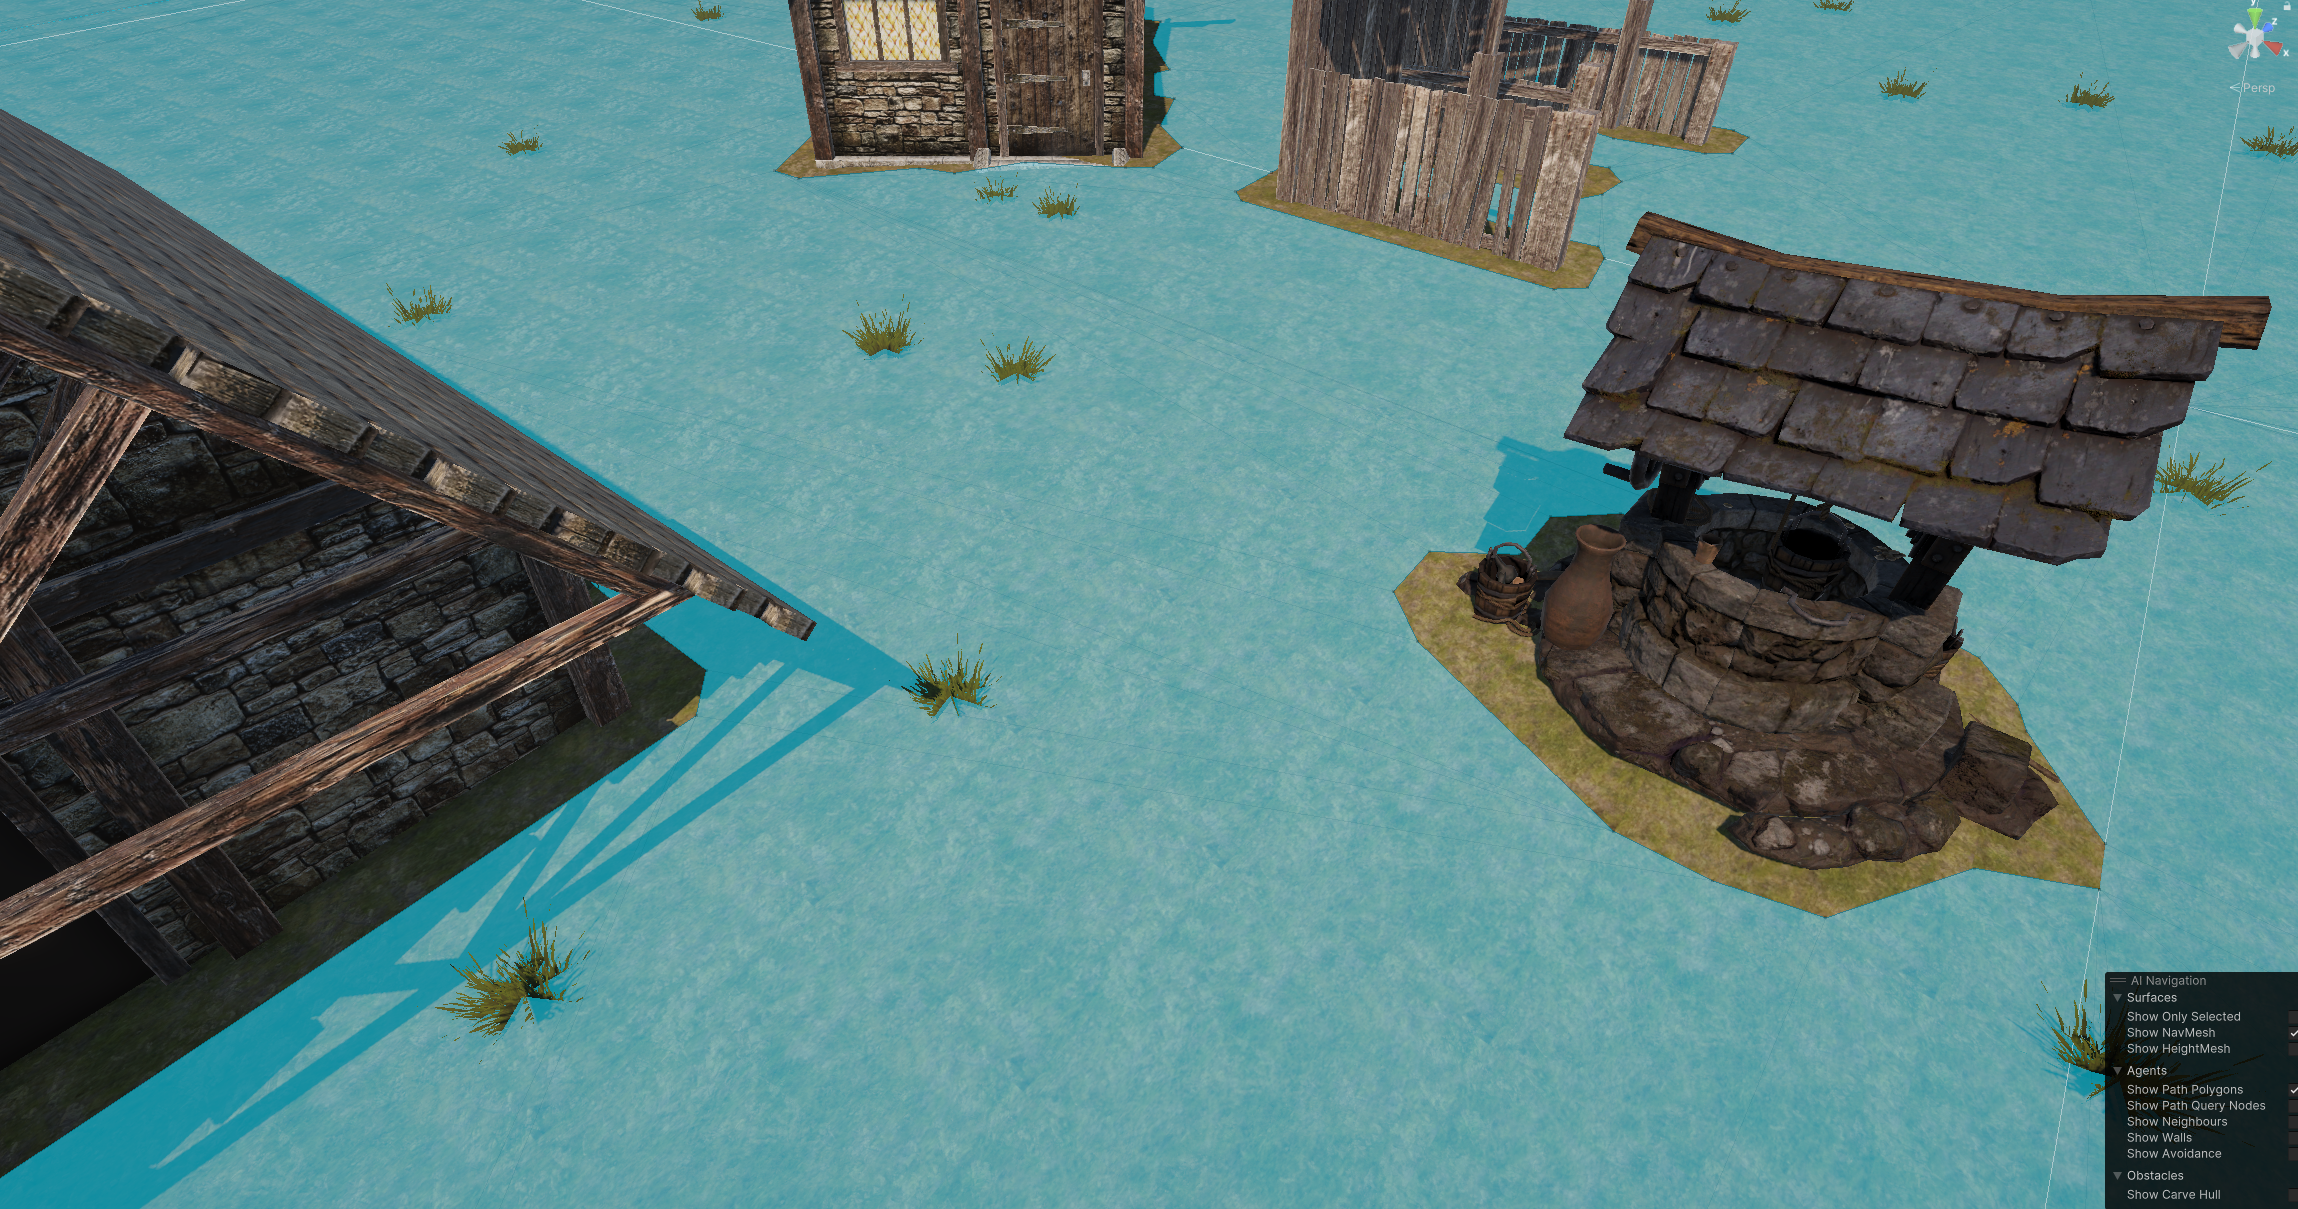
\includegraphics[width=0.9\textwidth]{images/navmesh.png}
    \caption{System nawigacji w Unity}
\end{figure}

Podsumowując system NavMesh istotnie upraszcza zadanie odnajdywania ścieżki, co pozwala na łatwe zaimplementowanie
realistycznych zachowań agentów sztucznej inteligencji. Znacznie ułatwia też zadanie tworzenia świata gry ze względu na automatyczny
sposób generowania danych nawigacyjnych.


\section{Struktury danych}
\section{Struktury danych}
\subsection{ScriptableObject (Bogna Lew)}
Silnik Unity umożliwia użytkownikom tworzenie klas typu ScriptableObject. Jest to struktura danych, która pozwala na
tworzenie wielu instancji klasy bez konieczności kopiowania danych. Poszczególne instancje współdzielą informacje, dzięki
czemu możliwe jest znaczące zoptymalizowanie użycia pamięci.

Do podstawowych zalet ScriptableObject należy możliwość wykorzystania go do tworzenia zasobów, które można by wykorzystać
w trakcie gry. Dzięki temu w prosty sposób można utworzyć szablony dla obiektów takich jak budowle, bronie i inne
przedmioty, które następnie można użyć do utworzenia jego instancji podczas rozgrywki.

\begin{figure}[h!]
    \centering
    \includegraphics[width=0.9\textwidth]{images/scriptableobjects.png}
    \caption{Przykład zasobów typu ScriptableObject.}
\end{figure}
\subsection{Protobuf (Bartosz Strzelecki)}\label{ss:protobuf}

Biblioteka \texttt{Protobuf} jest wydajnym i uniwersalnym rozwiązaniem przystosowanym do serializacji
danych. Służy do zdefiniowania formatu przechowywanych informacji, który jest neutralny dla platformy.
"Protocol Buffers zapewniają format serializacji dla pakietów o typowanych i ustrukturyzowanych danych o rozmiarze do
kilku megabajtów. Format nadaje się zarówno do efemerycznego ruchu sieciowego, jak i długoterminowego przechowywania
danych. Protocol Buffers można rozszerzyć o nowe informacje bez pozbawienia ważności istniejących danych lub
konieczności aktualizacji kodu." \cite{protobuf}.
W swojej istocie \texttt{Protobuf} definiuje niezależny od języka programowania schemat opisu interfejsu,
który pozwala na określenie struktury danych za pomocą prostej i intuicyjnej składni.
Elastyczność komponentu \texttt{Protobuf} wykracza poza proste struktury danych, oferując obsługę złożonych typów danych,
pól opcjonalnych i powtarzalnych,
a także struktur zagnieżdżonych. Dodatkowo udostępnia narzędzia do generowania kodu,
które automatycznie tworzą implementację specyficzną dla danego języka, ułatwiając pracę programistom.


\chapter{Projekt systemu}\label{chap:projekt}

W tym rozdziale został przedstawiony zamysł członków zespołu na opracowywaną grę. Stanowi on opis pożądanych rezultatów,
do których zespół będzie dążyć w trakcie implementacji. Kolejno zostały opisane oczekiwane działanie poszczególnych
mechanik, z których będzie się składał ostateczny produkt. 

\section{Organizacja (Bartosz Strzelecki)}\label{s:org}
W tym podrozdziale przedstawiono harmonogram prac, wraz z ich przewidywanym terminem realizacji.
Ponadto zaprezentowano skład zespołu projektowego, kompetencje ich członków oraz podział zadań.
\subsection{Główne etapy projektu}
\begin{center}
  \begin{tabular}{| m{30em} | m{12em}|} 
  \hline
  Etap & Termin realizacji \\
  \hline\hline
  Wybór i analiza konkretnego kontekstu historycznego. & Kwiecień 2023 \\
  \hline
  Syntetyczny opis modelu postrzegania przestrzeni na podstawie dzieł pisanych, architektury i sztuki. & Kwiecień — Maj 2023 \\
  \hline
  Przegląd rozwiązań stosowanych w grach strategicznych z wybranego okresu oraz dodatkowo mechanizmów z innych gier, które mogłyby być zaadoptowane na potrzeby projektu. & 2, 3 kwartał 2023 \\
  \hline
  Opracowanie fabuły, selekcja postaci i wydarzeń, a także określenie zakresu autonomii świata gry oraz możliwości modyfikowania go przez gracza. & Czerwiec 2023 \\
  \hline
  Opracowanie szczegółowej koncepcji i projektu gry, w tym projekt mechanizmów zawartych w prototypie. & Lipiec 2023 \\
  \hline
  Implementacja poszczególnych funkcjonalności gry. & 4 kwartał 2023 \\ 
  \hline
  Testowanie, weryfikacja założeń i walidacja. & Listopad — Grudzień 2023 \\
  \hline
  Stworzenie dokumentacji przeprowadzonych prac. & 3, 4 kwartał 2023 \\
  \hline
\end{tabular}
\end{center}
Przewidywany termin zakończenia prac nad projektem to grudzień 2023 roku.
\begin{figure}[htbp]
    \centering
    \includegraphics[width=1\textwidth]{uml/Harmonogram}
    \caption{Harmonogram przedstawiony w postaci diagramu gantt.}
\end{figure}
\section{Skład zespołu projektowego}
\begin{center}
  \begin{tabular}{ m{10em} m{10em} m{10em} m{10em} }
    Imię i nazwisko & Bogna Lew & Zofia Sosińska & Bartosz Strzelecki \\
    Numer indeksu & 184757 & 184896 & 184529 \\
    %%Kompentencje & Posiada & Posiada & Posiada \\
    Zadania & System budowania, sterowanie postacią & Interfejs użytkownika & Sztuczna inteligencja postaci\\
  \end{tabular}
\end{center}

\section{Analiza i specyfikacja wymagań (Bogna Lew, Zofia Sosińska)}\label{s:wymagania}
W niniejszej sekcji przedstawiono specyfikę wymagań funkcjonalnych, pozafunkcjonalnych oraz tych, wynikających z
głównych założeń projektu. Dodatkowo zawiera ona diagramy przypadków użycia, maszyny stanów oraz klas prototypowej gry.

\subsection{Specyfika wymagań wynikających z założeń projektu}
Z punktu widzenia projektu kluczowe jest jak najdokładniejsze oddanie realiów historycznych przy jednoczesnym
uwzględnieniu jakości rozgrywki gracza oraz cech charakterystycznych dla gier typu RTS. Z założeń wynika, że fabuła
gry powinna zostać osadzona w czasach sprzed wielkich odkryć geograficznych. Na tej podstawie zostały zdefiniowane
dodatkowe wymagania, które powinien spełniać prototyp.

Gra powinna zawierać:
\begin{itemize}
  \item sposób nawigacji jak najdokładniej odpowiadający temu stosowanemu w wybranej epoce,
  \item postacie:
  \begin{itemize}
    \item stylistycznie pasujące do realiów historycznych,
    \item wykorzystujące słownictwo adekwatne do czasów, w których osadzona jest gra,
    \item jak najlepiej oddawające światopogląd w danych czasach,
    \item stosujące oręż typowy dla wybranej epoki.
  \end{itemize}
  \item budowle stylistycznie odpowiadające wybranej epoce,
  \item sposób komunikacji z postaciami imitujący ten stosowany w danych czasach.
\end{itemize}

Dodatkowo po konsultacjach z pomysłodawcą projektu wyniknęło, że prototyp gry nie ma być typową grą z gatunku strategii
czasu rzeczywistego, a jego hybrydą z gatunkiem komputerowych gier fabularnych.

\subsection{Wymagania funkcjonalne}\label{ss:fun}
Niniejsza sekcja skupia się na określeniu wymagań funkcjonalnych, które powinien spełniać prototyp gry.

Gra powinna oferować możliwość:
\begin{itemize}\label{list:fun}
  \item uruchomienia nowej gry,
  \item sterowania postacią gracza,
  \item nawigacji w świecie gry,
  \item wchodzenia w interakcję z postaciami niezależnymi,
  \item przyjmowania zleceń od postaci niezależnych,
  \item najmowania postaci wojowników,
  \item wydawania komend wynajętym postaciom,
  \item zlecania budowy,
  \item zdobywania zasobów,
  \item odczytu wybranego stanu gry z komputera użytkownika,
  \item zapisu aktualnego stanu gry lokalnie na komputerze użytkownika.
\end{itemize}

\subsection{Wymagania pozafunkcjonalne}\label{ss:nonfun}
W tej sekcji zostały przedstawione wymagania pozafunkcjonalne projektu.

Gra powinna umożliwiać:
\begin{itemize}\label{list:nonfun}
  \item rozgrywkę w trybie offline,
  \item działanie na urządzeniach z systemem Windows lub Linux,
  \item dostosowywanie rozmiaru do wielkości ekranu komputera użytkownika,
  \item obsługę klawiatury oraz myszy,
  \item działanie w czasie rzeczywistym.
\end{itemize}

\subsection{Diagram przypadków użycia}\label{ss:usecase}
Niniejsza sekcja przedstawia diagram przypadków użycia dla głównych funkcjonalności, które będzie zawierać prototypowa gra.
Opisuje on przewidywane usługi oferowane przez poszczególne mechaniki programu.

Jedną z głównych akcji, które gra udostępni będzie wydanie rozkazów przyjaznym jednostkom. Polegać będzie ona na poinformowaniu
wojowników przez gracza jaką czynność powinni w danym momencie wykonać. Kolejną możliwością będzie zlecenie budowy, czyli
zlecenie budowniczemu wybudowania wybranego obiektu w określonym przez gracza miejscu. Ponadto użytkownik
będzie mógł przeprowadzać rozmowy z postaciami niezależnymi. Oznacza to, że będzie mógł zainicjować z nimi dialog i
następnie kształtować jego przebieg poprzez wybieranie swojej odpowiedzi z opcji proponowanych przez grę.

\begin{figure}[!htbp]
    \centering
    \includegraphics[width=1.0\textwidth]{images/diagrams/usecase.jpg}
    \caption{Diagram przypadków głównych mechanik gry.}\label{fig:usecases_d}
\end{figure}
\FloatBarrier

\subsection{Diagram stanów}\label{ss:state}
W tym podpunkcie został przedstawiony diagram stanów prototypowej gry, który ukazuje jej przewidywany sposób działania.
Prezentuje on podstawowe stany, w których może się znaleźć system gry.

Do podstawowych stanów należą "Menu główne" oraz "Rozgrywka". Pierwszy z nich oznacza, że program został uruchomiony, a
gracz wyświetla panel główny. Z tego stanu możliwe jest przejście do stanów "Odczytanie stanu gry" bądź "Utworzenie
nowej gry", które to powodują rozpoczęcie gry z zapisu lub od początku.

Stan "Rozgrywka" jest stanem złożonym i określa, że gra została rozpoczęta. W jego skład wchodzą przede wszystkim takie
stany, jak "Interakcja z postacią niezależną", w którym program się znajdzie, gdy gracz rozpocznie dialog z postacią w grze,
czy "Zarządzanie jednostkami", który to oznacza, że użytkownik wydaje rozkazy swoim wojownikom.

Diagram stanów został przedstawiony na rysunku \ref{fig:states_d}.

\begin{figure}[!htbp]
    \centering
    \includegraphics[width=1.0\textwidth]{images/diagrams/state.jpg}
    \caption{Diagram stanów gry.}\label{fig:states_d}
\end{figure}
\FloatBarrier

\subsection{Diagram klas}\label{ss:class}
W tej sekcji został pokazany uproszczony diagram klas (rys. \ref{fig:classes_d}), przedstawiający główne elementy gry.
Obrazuje podstawową strukturę tworzonego systemu oraz zależności pomiędzy poszczególnymi komponentami.

Do najważniejszych klas należą "Interfejs użytkownika", "Mechanizm interakcji z postaciami", "Mechanizm zarządzania
jednostkami" oraz "Mechanizm budowania". Obrazują one podstawowe komponenty gry, których głównym zadaniem jest zarządzanie
poszczególnymi mechanikami. "Interfejs użytkownika" jest odpowiedzialny za interakcję z graczem oraz pomaganie mu w
trakcie rozgrywki. Pozostałe trzy kolejno pozwalają graczowi na prowadzenie dialogów z postaciami
niezależnymi, wydawanie komend jego zaprzyjaźnionym jednostkom oraz budowanie obiektów.
\begin{figure}[!htbp]
    \centering
    \includegraphics[width=1.0\textwidth]{images/diagrams/class.jpg}
    \caption{Diagram klas gry.}\label{fig:classes_d}
\end{figure}

\section{Opis świata gry (Bogna Lew)}
Fabuła wytwarzanej gry ma zostać osadzona w realiach wczesnośredniowiecznych. Została ona zainspirowana Celtami, których
w tym okresie można było spotkać głównie w Irlandii. Z tego powodu mapa świata gry będzie prezentować górzystą wyspę na
której gracz będzie mógł znaleźć niewielką wioskę oraz obozowiska.

Gracz będzie mieć do dyspozycji swoją postać, którą będzie mógł bezpośrednio sterować. W trakcie gry użytkownik będzie
mógł spotkać postaci niezależne z którymi będzie mógł wchodzić w interakcje i które mogą mu zlecić wykonanie zadania.
W ich realizacji będą mu pomagać jednostki z którymi się zaprzyjaźni w trakcie rozgrywki i którym będzie mógł wydawać
komendy zgodnie z ich typem. Dodatkowo w trakcie eksploracji świata natrafi na nieprzyjazne postacie z którymi
będzie toczyć walki. Grę urozmaicą postaci zwierząt, które mogą być neutralne, bądź agresywne wobec gracza.

Gra będzie udostępniać trzy podstawowe surowce za które gracz będzie mógł budować budynki. Gracz będzie mógł pozyskiwać
zasoby na dwa sposoby. Pierwszym z nich jest wykonywanie zadań za które może uzyskać nagrody w postaci pewnej ilości
surowców. Kolejnym sposobem jest budowanie obiektów, które zajmują się produkcją zasobów, przynosząc graczowi stały
dochód.

\section{Poruszanie postacią (Bogna Lew)}
Podstawową mechaniką, którą będzie oferować implementowana gra jest sterowanie postacią przez gracza. Użytkownik będzie
mieć do dyspozycji jedną postać, którą będzie bezpośrednio zarządzać. Umożliwi mu ona przede wszystkim eksploraację
świata oraz walkę z przeciwnikami.

Poruszanie postacią będzie analogiczne jak w grze The Elder Scrolls V: Skyrim. Gracz będzie mógł przemieszczać się
do przodu, do tyłu, na boki oraz na ukos. Sterowanie będzie możliwe za pomocą klawiszy  “w”, “a”, “s” oraz “d”.
Dodatkowo użytkownik będzie mieć możliwość obracania postaci, a tym samym zmiany kierunku w którą jest zwrócona poprzez
przemieszczanie myszy. Ponadto, gra udostępni możliwość przesunięcia kamery po łuku do góry bądź do dołu.

Kolejnym aspektem jest walka. Użytkownik będzie mógł wykonać atak porzez naciśnięcie prawego przyciku myszy. Postać
gracza będzie mogła wykonywać wyłącznie ataki bronią białą, która zostanie dobyta w momencie gdy znajdzie się on w walce.
\section{Menu główne (Zofia Sosińska)}\label{chap:menu_main}
Pierwsze co zobaczy użytkownik po włączeniu programu to menu główne, więc jego zadaniem będzie oddanie klimatu programu,
umożliwienie rozpoczęcia rozgrywki oraz zamknięcie aplikacji.
Projekt zakłada, że menu główne udostępni kluczowe funkcjonalności za pomocą przycisków:
\begin{itemize}
    \item rozpoczęcia nowej gry,
    \item wczytania zapisanej gry,
    \item wyjścia z programu.
\end{itemize}

Przycisk wczytania gry będzie musiał pozwolić na wybranie pliku zapisu. W tym celu przewiduje się wyświetlenie listy
z możliwością przewijania treści za pomocą suwaka. Jej elementami będą przyciski z nazwą zapisu, których naciśnięcie przeniesie 
użytkownika do konkretnego stanu gry.

\begin{figure}[htbp]
    \centering
    \includegraphics[width=0.8\textwidth]{images/ui/ui_prooj_menu.jpg}
    \caption{Projekt menu głównego.
    }\label{fig:compass}
\end{figure}

\section{Interfejs użytkownika (Zofia Sosińska)}\label{chap:ui}
Projekt interfejsu użytkownika przewiduje tryb podstawowy z zawsze widocznymi elementami oraz dynamicznie pojawiające się okna, wywoływane za pomocą konkretnych klawiszy. 
 Zadaniem każdej składowej będzie odzwierciedlenie pewnego fragmentu aktualnego stanu wiedzy granej postaci z naciskiem na najpotrzebniejsze w danej chwili informacje. Przewidziane są:
 \begin{itemize}
    \item menu stawiania budynków; 
    \item menu wydawania komend;
    \item menu zapisu;
    \item informacja o możliwej interakcji;
    \item dziennik z zadaniami;
    \item ekran końca gry.
\end{itemize}
	
\subsection{Interfejs podstawowy}
Interfejs podstawowy przewiduje funkcje, takie jak pokazanie:
\begin{itemize}
    \item aktualnego czasu w grze, aby stworzyć iluzję upływającego czasu w świecie gry; 
    \item surowców i funduszy, aby użytkownik nie był obarczony kalkulacjami przy każdym zakupie lub przypływie zasobów;
    \item kompasu, aby ułatwić nawigację;
    \item stan zdrowia gracza, aby zasygnalizować mu, czy przypadkiem nie rozsądniejsze będzie wycofanie się z potyczki;
    \item etap, na którym są przypisane graczowi zadania, aby przypomnieć mu, że na takowe się zgodził.
\end{itemize}
Inspiracją dla górnego paska z informacjami jest ten użyty w grze Warcraft 3 (por. \ref{c:elem_ui}). Prostota i surowość stylu będą współgrać z klimatem gry.

W naszej grze skupimy się jednak na tym, aby interfejs użytkownika zabierał jak najmniej miejsca. Dlatego też projekt zakłada, że poszczególne obiekty nie będą ze sobą połączone, a jedynie “dryfować” w przestrzeni.
Jako ważny element tej części UI zawarty zostanie kompas, wzorowany na tym z gry The Elder Scrolls V: Skyrim (por. \ref{chap:skrm}).
\begin{figure}[htbp]
    \centering
    \includegraphics[width=0.9\textwidth]{images/ui/ui_proj_ogolne.jpg}
    \caption{Projekt interfejsu podstawowego UI.
    }\label{fig:ui_main}
\end{figure}
 
\subsection{Menu stawiania budynków}
Menu stawiania budynków będzie obrazować wiedzę i spostrzeżenia głównej postaci przy budowaniu nowej budowli. Docelowym miejscem ukazania się informacji będzie 
dół ekranu, aby interfejs nie zasłaniał użytkownikowi zbyt dużo przestrzeni. Graczowi ukaże się lista dostępnych budynków oraz odpowiednie komunikaty w wypadku, gdy 
nie można będzie dokonać zakupu, czy postawienia. Inspiracją do przedstawienia tych informacji zostanie rozwiązanie gry Orcs must die! (por. \ref{c:elem_ui}).
\begin{figure}[htbp]
    \centering
    \includegraphics[width=0.9\textwidth]{images/ui/ui_proj_budowanie.jpg}
    \caption{Projekt menu stawiania budynków.
    }\label{fig:ui_bud}
\end{figure}
\FloatBarrier

\subsection{Menu wydawania komend}
Po zdobyciu towarzyszy broni, kluczowe będzie udostępnienie mechaniki sterowania nimi. Zrealizowane to zostanie za pomocą menu wydawania komend.
Projekt przewiduje wyświetlenie listy dostępnych komend i klawiszy, po których naciśnięciu, konkretna opcja zostanie wybrana. 
Źródłem pomysłu jest interfejs zaprojektowany w grze Mount\&Blade (por. \ref{chap:mb}).

\begin{figure}[htbp]
    \centering
    \includegraphics[width=0.9\textwidth]{images/ui/ui_proj_walka.jpg}
    \caption{Projekt menu wydawania komend.}\label{fig:cmd_menu}
\end{figure}
\FloatBarrier

\subsection{Menu zapisu}
Aby umożliwić zapis gry przygotowane zostanie specjalne dla tego zadania menu, wyświetlane na środku ekranu. Najważniejszą informacją 
umiejscowioną na nim będzie nazwa pliku, aby gracz mógł później go odnaleźć.
\begin{figure}[htbp]
    \centering
    \includegraphics[width=0.9\textwidth]{images/ui/ui_proj_zapis.jpg}
    \caption{Projekt menu zapisu.}\label{fig:men_zap}
\end{figure}
\FloatBarrier

\subsection{Informacja o możliwej interakcji}
W programie przewidziane są postacie i przedmioty interaktywne. Aby zasygnalizowć mu zaistniałą możliwość podjęcia pewnej akcji, 
gra powinna mu wyświetlić stosowny komunikat. Wybranie widocznego miejsca będzie istotne, ponieważ grafika zniknie,
jak tylko interakcja przestanie być możliwa. Tudzież kluczowe będzie wybranie takiej lokalizacji, aby komunikat zwrócił uwagę gracza nawet, 
jeśli wyświetlony będzie tylko przez krótką chwilę. Za najwłaściwsze umiejscowienie wybrano środek górnej części ekranu, zaraz
pod bazowym interfejsem.
    \begin{figure}[htbp]
    \centering
    \includegraphics[width=0.9\textwidth]{images/ui/ui_prooj_interakcja.jpg}
    \caption{Projekt grafiki informującej o możliwym rozpoczęciu rozmowy.}\label{fig:rozmow}
\end{figure}
\FloatBarrier

\subsection{Dziennik z zadaniami}
Projektanci systemu zakładają, że niektóre postacie interaktywne będą mogły zlecić graczowi zadanie. Jeśli użytkownik przyjmie wiele zleceń,
to zapamiętanie wszystkich szczegółów może stać się kłopotliwe. Dlatego projekt systemu przewiduje udostępnienie mechaniki dziennika, w którym 
pojawią się informacje o rozpoczętych zadaniach. Na przygotowanej grafice każde z nich będzie miało własne okno ze streszczeniem. Użytkownik 
będzie mógł je przeglądać posługując się suwakiem.
\begin{figure}[htbp]
    \centering
    \includegraphics[width=0.9\textwidth]{images/ui/ui_proj_dziennik_zadan.jpg}
    \caption{Projekt dziennika z aktualnie zaczętym i nieukończonym zadaniem.}\label{fig:end_sc}
\end{figure}
\FloatBarrier

\subsection{Ekran końca gry}
Gracz, po wykonaniu pewnych kroków, może doprowadzić grę do stanu końcowego. W takim wypadku przewidziane jest wyraźne tego zasygnalizowanie przez program.
Przewiduje się zaprojektowanie specjalnego ekranu końca gry. W tym celu użytkownikowi zostanie wyświetlona klarowna informacja o aktualnym stanie rzeczy oraz instrukcja,
co zrobić dalej. Dodatkowo, aby wzmocnić przekaz, cały ekran zostanie przyciemniony.
\begin{figure}[htbp]
    \centering
    \includegraphics[width=0.9\textwidth]{images/ui/ui_prooj_koniec_gry.jpg}
    \caption{Projekt ekranu końca gry.}\label{fig:end_sc}
\end{figure}
\FloatBarrier

\section{Nawigacja. Zofia Sosińska}\label{chap:naw}

    Kluczowym dla gry założeniem jest ułatwienie graczowi wczucia się w realia świata, w którym się znajduje. Jako jeden z głównych warunków pogłębienia immersji uwypuklono brak implementacji mapy, na której gracz widziałby świat. W ten sposób nie upraszczamy mu poruszania się i odnajdywania lokacji tak, jak i człowiek w realnym świecie w czasach średniowiecznych nie kierował się zapisanymi na kartce kartograficznymi obrazami, ale własną i zdobytą od innych wiedza o otaczającym go terenie. 
    Jedyną pomocą, jaką otrzyma gracz, będzie pasek obrazujący pole widzenia granej postaci. Pierwszą rolą narzędzia będzie pokazanie kierunku świata, który znajduje się w polu widzenia gracza. Zakładamy, że grana postać potrafi sama taką, informację odczytać chociażby z położenia Słońca. Nie jest to więc sztucznie upraszczająca rozgrywkę mechanika, a jedynie odciążenie użytkownika kompasem. 
    Kolejną informacją na omawianym polu będzie miejsce w którym znajduje się przeciwnik. Dotyczy to antagonistów widocznych w polu widzenia, jak i ukrytych za ścianą. Druga część będzie logicznie możliwa dzięki specjalnej umiejętności widzenia wrogów za przeszkodą zaimplementowanej dla postaci druida. Po przyłączeniu takiej osoby do drużyny użytkownik może poprosić przyjaciela o użyczenie mu swej mocy.

\begin{figure}[htbp]
    \centering
    \includegraphics[width=0.9\textwidth]{images/ui/compass.png}
    \caption{Wizualizacja przypadku, w którym gracz patrzy centralnie na północ. Delikatnie na jego prawo znajduje się dwóch przeciwników za ścianą, podświetlonych specjalną umiejętnością druida.
    }\label{fig:compass}
\end{figure}


\section{Mechanizm budowania (Bogna Lew)}\label{s:build_proj}
Inspiracją do implementacji tego mechanizmu jest gra \textit{Warhammer 40,000: Dawn of War} (por. \ref{s:budowanie}). Do pożądanych
efektów, które ten tytuł zapewnia, należą walidacja terenu oraz wymuszanie poniesienia kosztów budowy. Dodatkowo
wytwarzana gra będzie implementować proces budowania analogicznie jak w \textit{Warhammer 40,000: Dawn of War}.

Najważniejszym aspektem implementowanego mechanizmu będzie walidacja terenu. Zostanie ona uzyskana poprzez wyświetlenie
podglądu budowli w trakcie umiejscawiania konstrukcji na mapie. Jeśli miejsce, w którym gracz chce postawić budynek jest
poprawne tzn. nie nachodzi na inne obiekty oraz teren jest odpowiedni, to pokazywany widok jest podświetlany na zielono,
w przeciwnym razie - na czerwono. Jest to efekt, który wytwarzana przez zespół gra będzie zawierać.

Kolejnym pożądanym efektem jest konieczność poniesienia przez użytkownika kosztów
wybudowania obiektu. W tym celu gra będzie monitorowała, czy gracz posiada wystarczającą ilość wymaganych zasobów, a w
przypadku niespełnienia tych warunków - blokowała możliwość budowy wybranego obiektu.

Dodatkowo budowa obiektu nie może być natychmiastowa, gdyż nie jest to zgodnie z rzeczywistością. Dlatego podobnie jak w
grze \textit{Warhammer 40,000: Dawn of War} każdy budynek będzie musiał zostać wybudowany przez dedykowaną do tego postać. Będzie
ona imitowała proces budowania i dopiero gdy ukończy to zadanie, dana budowla zacznie przynosić graczowi korzyści.

\section{Sterowanie jednostkami, podążanie za główną postacią (Zofia Sosińska)}\label{chap:sjpzgp}
Na samym początku gry postać gracza pojawia się sama i jest jedynym obiektem, którym gracz może sterować.
Kontroluje, gdzie postać idzie, jak walczy oraz z kim rozmawia. Z biegiem czasu gra będzie jednak naciskać na formowanie drużyny,
ponieważ pokonywanie wielu przeciwników w pojedynkę będzie się stawało zbyt trudne. Pojawia się w takim momencie potrzeba 
zaimplementowania funkcjonalności zarządzania wieloma postaciami.

Stworzenie mechaniki poruszania się i oddziaływania na otaczający świat dla jednej postaci wydaje się proste i intuicyjne, ale kierowanie wieloma osobami już nie. 
Bez wprowadzenia zmian, używając jednego sposobu dyrygowania wszystkimi jednostkami tak samo, gra będzie prędko męczyć gracza.
Dla czynności małoznaczących, takich jak przemieszczenie drużyny w konkretne miejsce, wprowadzi monotonię i czasochłonność.
Każdą postać należy wybrać i przemieścić ją w konkretne miejsce. Kilka kliknięć przy jednej postaci jest akceptowalne, ale przy kilku wprowadzi to ogromne opóźnienia.

Jeszcze gorsze skutki pokazałyby się podczas walki. Szybkie przeskakiwanie pomiędzy postaciami podniosłoby zauważalnie trudność gry.
Poruszanie się jedną postacią i zabijanie przeciwników nie ma sensu, gdy reszta drużyny jest bita i nie może się obronić, ponieważ gracz musi się przełączyć na inną postać,
aby ta wykonała ruch. 

Z tego powodu potrzebny jest algorytm odpowiadający za właściwe poruszanie się pobocznych postaci.
Tworzona gra będzie dopuszczała małe, kilkunastoosobowe drużyny z przywódcą - postacią grywalną przez użytkownika - na czele.
Podczas walki graczowi pokażą się możliwe do wydania polecenia oraz specyfikacja, jakiej grupy mają one dotyczyć.
Za pomocą określonych klawiszy klawiatury będzie on mógł kontrolować zachowanie kompanów.

Po rozwiązaniu problemu mechaniki sterowania jednostkami w walce nie można przeoczyć samego poruszania się oraz interakcji ze światem.
Najprostszym rozwiązaniem będzie implementacja mechanizmu, według którego drużyna, po wykryciu znacznego przemieszczenia się przywódcy, sama będzie za nim podążać.
Kompani nie będą też mieli opcji samodzielnej interakcji ze światem, co sprawi, że poza walką zostaną jedynie biernymi obserwatorami.
\section{System dialogów (Bartosz Strzelecki)}

System dialogów jest podstawową metodą, którą gracz będzie wykorzystywał, aby pozyskać informacje  o świecie oraz celach misji.
Gracz może inicjować konwersacje z postaciami niezależnymi, po czym zostaną mu zaproponowane opcje sposobu prowadzenia rozmowy.
W zależności od wybranych opcji dialogowych gracz może się spodziewać różnych konsekwencji.
"Postacie niezależne (NPC) w grach są jednym z najbardziej złożonych i uniwersalnych sposobów pośredniego prowadzenia graczy, który może przybierać różne formy"\cite{projektowanie_gier}


\href{https://assetstore.unity.com/packages/tools/utilities/dialogue-editor-168329}{Dialogue Editor} autorstwa Grasshop Dev jest prostym narzędziem pozwalającym na szybkie dodawanie i modyfikację dialogów.
Zawiera zestaw elementów ułatwiających wdrożenie systemu do projektu oraz udostępnia struktury danych wykorzystywanych do tworzenia interfejsu użytkownika.
Podczas rozmowy z postaciami niezależnymi gracz będzie mógł pozyskać informację o geografii świata, możliwych zagrożeniach oraz zadaniach do wykonania. 
Podobne systemy występują w grach takich jak Pillars of Eternity oraz w grach z serii Mass Effect. (por. \ref{chap:dialogi})


\section{Sztuczna inteligencja (Bartosz Strzelecki)}
W przypadku implementacji mechanizmów sztucznej inteligencji przeciwników będziemy się inspirować trybami kampanii w grach Warcraft III oraz Starcraft II (por. \ref{s:ai_wpr}). 
Na mapie będą rozsiane punkty, w których będą pojawiać się przeciwnicy. 
Tak długo, jak drużyna gracza jest poza zasięgiem, wrogowie pozostają nieaktywni. 
Aktywni przeciwnicy zachowują się zgodnie z ich archetypem (klasą postaci) oraz pozostają aktywni tak długo, jak drużyna gracza jest w zasięgu. 
Zdezaktywowani przeciwnicy wracają do swojego oryginalnego stanu. Gracz będzie napotykał tego typu obozowiska przede wszystkim w trakcie eksploracji świata. 
Innym planowanym przykładem implementacji sztucznej inteligencji przeciwników jest model, w którym jednostki wroga poruszają się z punktu początkowego w stronę bazy gracza. 
Jeśli podczas swojej podróży napotkają drużynę gracza, wtedy niezwłocznie zmieniają swój cel ataku.
Będziemy wyróżniać trzy archetypy jednostek w zależności od sposobu walki (bliski zasięg, średni zasięg, daleki zasięg). 
Postacie walczące na bliski zasięg mają na celu podejście w stronę najbliższego przeciwnika i wykonać atak. 
Jednostki średnio zasięgowe w momencie, w którym najbliższy przeciwnik jest odpowiednio daleko, wykonują atak dystansowy, 
w przeciwnym wypadku zachowują się tak jak jednostki walczące w zwarciu. 
Postacie  dalekodystansowe dokonują ataków dystansowych w kierunku najbliższego przeciwnika, natomiast uciekają, gdy ten podejdzie zbyt blisko.



\section{Widzenie przez ściany (Bartosz Strzelecki)}\label{s:wid_proj}

Do umiejętności wykorzystywanych przez gracza będzie należeć zdolność widzenia przeciwników oraz innych istotnych obiektów przez przeszkody.
Gracz po wciśnięciu przycisku przez krótki okres będzie w stanie zobaczyć sylwetki przeciwników znajdującymi się w jego polu widzenia.
Rozwiązanie jest inspirowane wcześniej wspomnianą grą \textit{Dead by Daylight} (por. \ref{chap:dbd}). Po pojawieniu się,
markery nie będą się poruszać za celem, lecz pozostać w tym samym miejscu przez czas trwania animacji.





\chapter{Implementacja}
Ten rozdział skupia się na zaprezentowaniu implementacji projektu w silniku Unity.
Przedstawia on wykorzystane metodyki i narzędzia wykorzystane do osiągnięcia określonych wymagań.
Jak również zawiera fragmenty wykorzystanych algorytmów i zrzuty ekranu reprezentujące efekty pracy.


\chapter{Podsumowanie}
\label{chap:summary}

% Bibliografia, ignorujemy overfull box, bo są długie URL
\hfuzz=50pt
\printbibliography[title=\bibliographyname]
\addcontentsline{toc}{chapter}{\bibliographyname}
\hfuzz=0pt

% Wykaz rysunków
\listoffigures
\addcontentsline{toc}{chapter}{\listfigurename}

% Wykaz tabel
\listoftables
\addcontentsline{toc}{chapter}{\listtablename}

\end{document}
